\documentclass[12pt]{article}
\usepackage[UTF8]{inputenc}
\usepackage[french]{babel}
\usepackage[T1]{fontenc}
\usepackage{hyperref}
\hypersetup{
    colorlinks=true,
    linkcolor=blue,
    filecolor=magenta,      
    urlcolor=cyan,
}
\usepackage{amsmath,amssymb,amsfonts}
\usepackage{graphicx}
\graphicspath{{figures/}}
\usepackage{amsmath}
\usepackage{fancyvrb}
\usepackage{geometry}
\usepackage{float}
\geometry{hmargin=2.0cm,vmargin=1.5cm}
\title{Rapport de stage - Master 1 MAPI3 2019/2020}
\author{Antoine Perrot}
\usepackage{framed,color,verbatim}
\usepackage{xcolor}
\definecolor{shadecolor}{rgb}{.95, .95, .98}
\usepackage{color, listings}

\setlength{\parindent}{0pt}
\newenvironment*{remerciements}{%
\renewcommand*{\abstractname}{Remerciements}
\begin{abstract}
}{\end{abstract}}

\newenvironment{code}%
   {\snugshade\verbatim}%
   {\endverbatim\endsnugshade}
   
\begin{document}
\begin{titlepage}

\newcommand{\HRule}{\rule{\linewidth}{0.5mm}} % Defines a new command for the horizontal lines, change thickness here

\center % Center everything on the page
 
%----------------------------------------------------------------------------------------
%	HEADING SECTIONS
%----------------------------------------------------------------------------------------

\textsc{\LARGE Université Paul Sabatier}\\[1.5cm] % Name of your university/college
\textsc{\Large M1 MAPI3 - Année scolaire 2019/2020}\\[0.5cm] % Major heading such as course name
\textsc{\large Stage du 27 avril au 31 juillet 2020 chez TEAMBER}\\[0.5cm] % Minor heading such as course title

\HRule \\[0.4cm]
{ \huge \bfseries Développement de fonctionnalités pour un logiciel de gestion de projet}\\[0.4cm] % Title of your document
\HRule \\[1.5cm]

\begin{minipage}{0.4\textwidth}
\begin{flushleft} \large
\emph{Auteur :} Antoine \textsc{Perrot} \\
\emph{Maître de stage :} Sébastien \textsc{Perrot} \\
\emph{Enseignant tuteur :}  Luca \textsc{Amodei} \\
\end{flushleft}
\end{minipage}





\vfill % Fill the rest of the page with whitespace

\end{titlepage}

\newpage
\textbf{\huge Remerciements}\\

J'aimerais remercier l'ensemble des enseignants qui ont été les miens à l'université Paul Sabatier, tout particulièrement lors de cette année 2019/2020 : messieurs Amodei, Malgouyres et Maréchal. Pour leur écoute et les connaissances qu'ils m'ont apportées je leur suis très reconnaissant.\\

Dans le contexte de ce stage, j'ai pu échanger régulièrement avec l'ensemble des membres de l'équipe Teamber afin de créer des fonctionnalités. Ils m'ont, par leur expérience, guidé dans mon travail afin de développer des fonctionnalités répondant à de réels besoins clients. Pour l'intérêt qu'ils ont accordé à mon travail, ainsi que pour l'accueil qu'ils m'ont offert dans leur équipe pendant ces 3 mois, je voudrais les remercier sincèrement.\\

\newpage
 
\tableofcontents






\newpage


\section{Introduction}
\subsection{Courte présentation de l'entreprise}
Le logiciel TEAMBER développé par l'entreprise du même nom est destinée à des entreprises de tailles humaines, relevant principalement des professions intellectuelles (architectes, avocats, bureau d'études...). \\
Les objectifs sont multiples : 
\begin{itemize}
\item fluidifier la communication au sein de l'entreprise.
\item permettre un meilleur suivi de l'avancement des tâches, des temps, dans l'entreprise.
\item avoir une vision à court et long termes de l'état de la situation économique de l'entreprise
\item permettre une meilleure organisation et répartition des tâches dans l'entreprise, afin de mieux se focaliser sur les tâches essentielles et éliminer toutes les potentielles perturbations venant dégrader la productivité.
\end{itemize}
\subsection{Visée du stage}
L'objectif de ce stage était le développement de fonctionnalités qui pourront être intégrées à la prochaine version de Teamber, qui devrait être achevée fin 2020. \\
Ces nouvelles fonctionnalités enrichiront le logiciel en répondant à de réels besoins des clients. Dans leur ensemble, elles contribueront pour l'entreprise qui les utilisera, à une plus grande efficacité au travail, en automatisant ou facilitant un certain nombre de tâches qui relèvent de la gestion et de l'organisation.

\newpage

\section{Première mission : aide à la classification de mails}

\subsection{Présentation de la mission}
Le premier objectif qui m'a été confié, a été le classification de mail selon leur catégorie. Explications : \\

L'utilisateur de TEAMBER, typiquement un membre d'un cabinet d'architecture, reçoit constamment des mails concernant différents projets, répertoriés dans Teamber.\\
Pour chacun de ces projets, l'on peut connaître ses différents paramètres, son état d'avancement etc. ainsi que l'ensemble des documents (appelés documents mais sont en fait des mails) interagissant avec ce projet.\\
Teamber n'ayant pas de boite mail intégrée, fait le pont avec le boite mail Outlook du l'utilisateur. Ainsi, quand un mail arrive dans la boite Outlook, quelques instants plus tard il arrive dans Teamber dans le répertoire "A traiter". Lorsque l'utilisateur classe un mail dans Outlook dans un dossier du repértoire Outlook, ce même mail est classé dans le dossier du même nom dans Teamber et à défaut supprimé. Réciproquement, si un mail est classé dans Teamber alors il est classé dans Outlook. L'arborescence des projet de Teamber est contenue dans celle de la boîte de réception Outlook.

L'intérêt principal de ma mission est de supprimer (ou de diminuer au maximum) une tâche chronophage et réberbative, et d'aller dans le sens d'une meilleure organisation générale.\\
En effet, classer les mails est indispensable pour beaucoup de clients Teamber, afin de rester organisé et ne pas être submergé par le flux constant de mails. Certaines personnes utilisent leur boîte mail comme "To-do list", mais dès que le flux devient trop important ce fonctionnement devient rapidement impossible, certaines études suggèrent même qu'à partir de 7 ou 8 mails, l'on est dépassé.\\
Cependant, si l'on veut resté organisé, mais que l'on a une cinquantaine de projets en cours, l'on passe alors énormément de temps à faire défiler son écran pour classer chaque mail.\\
L'idéal serait alors qu'une fois le mail sélectionné, le projet correspondant suggéré par Teamber soit accessible immédiatement. Nous tenterons donc de suggérer le bon projet à chaque nouveau mail.



\subsection{Collecte des données}

Après être allé collecter les données dans une base de données Drupal, les avoir recoupées dans Microsoft Access, j'ai pu obtenir des données propres afin de pouvoir travailler dans python.\\

Voici ce à quoi ressemble les données :
\begin{figure}[H]
\begin{center}
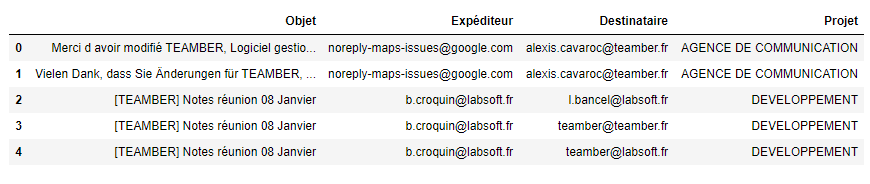
\includegraphics[width=0.99\textwidth]{donneesmail}
\end{center}
\end{figure}
\newpage
\subsection{Formatage des données}

Pour transformer les données textuelles en vecteur de nombre, on utilise l'objet \textbf{TfidfVectorizer }qui effectue un décompte des mots, calcule leur Inverse Document Frequency et leur attribue un score Tf-idf.\\

Lors de l'entraînement du modèle, on appellera cet objet avec l'extension \textbf{.fit\_transform(X\_train)} d'abord pour qu'il transforme les données textuelles en vecteurs de $\mathbb{R}^n$ mais aussi pour qu'il se constitue un vocabulaire (ensemble de mots rencontrés). En effet, lorsqu'il s'agira d'effectuer des prédictions sur \textbf{X\_test}, il faut que celui-ci ait les mêmes dimensions. La taille de ce vecteur est exactement le nombre de mots du vocabulaire. On appellera l'extension \textbf{.transform(X\_test)} afin de transformer les données de test correctement.


\subsection{Choix du modèle}
Après avoir transformé nos données textuelles et séparé les données en train/test dans les proportions 80/20, on entraîne différents modèles afin de comparer les scores et choisir le meilleur :
\begin{code}
models = [RandomForestClassifier(n_estimators=500, max_depth=5, random_state=0),
          LinearSVC(),
          MultinomialNB()]

print("#mails pour training :",X_train_vect.shape[0],'\n#projets :',y_train.max())
for model in models:
    model_name = model.__class__.__name__
    model.fit(X_train_vect,y_train)
    print('Accuracy',model_name,':',model.score(X_test_vect,y_test))
\end{code}


\begin{verbatim}
OUTPUT :
#mails pour training : 135806 
#projets : 133
Accuracy RandomForestClassifier : 0.3800954288407163
Accuracy LinearSVC : 0.9151154571159283
Accuracy MultinomialNB : 0.8030749293119699
\end{verbatim}

On retient donc le modèle LinearSVC qui est de loin le meilleur avec 91\% de prédictions correctes.

\paragraph{Rermarque :} on a essayé d'augmenter la précision en constituant un top 3 pour un mail donné. On a constaté que le bon projet était dans ce top 3 dans 92\% des cas. En prenant en compte le fait qu'il faudra intégrer cette fonctionnalité de prédiction à la boîte mail (menu déroulant pour le top 3 contre simple ligne pour proposition unique) et que le gain de précision n'était pas significatif, il a été décidé de ne pas retenir l'option du top 3.


\newpage
\section{Deuxième mission : optimisation de la répartition des tâches}
\textbf{But :} répartir le plus intelligemment possible le travail (les tâches)entre les utilisateurs lors de la planification d'un sprint.\\

\textbf{Dans Teamber, une tâche :}
\begin{itemize}
\item fait référence à une unique compétence.
\item fait référence à un unique projet.
\item a une durée.
\end{itemize}
Plus précisément, on va répartir les heures de travail contenues dans les tâches. Ainsi, une première personne pourra réaliser 3h d'une tâche et une seconde 4h de cette même tâche, qui faisait initialement 7h.\\


\textbf{Dans Teamber, un utilisateur :}
\begin{itemize}
\item a des compétences (matrice de compétences).
\item dispose d'une quantité maximale (en heure) de travail qu'elle peut réaliser au cours du sprint à venir.
\item est impliqué dans un ensemble de projets.
\end{itemize}


\begin{figure}[H]
\caption{Exemple de matrice de compétences}
\begin{center}
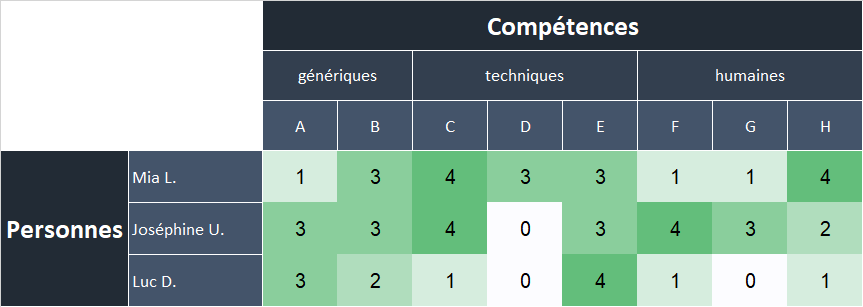
\includegraphics[width=0.75\textwidth]{matrice comp}
\end{center}
\end{figure}

Voici un exemple de matrice de compétences trouvé sur google image, chez Teamber les scores sont compris entre 0 (ne sait pas faire) et 3 (maîtrise parfaite, apte à la formation) mais le principe reste le même.


On a donc un ensemble de tâches avec des durées $d_1,..., d_{n}$ et un ensemble de personnes $p_1,..., p_{m}$ sur lesquels répartir ces durées.
Notons $u_1,..., u_{m}$ le nombre d'heures maximale que peuvent effectuer chacune des personnes.\\

\newpage
\subsection{Politique d'assignation}
Notre première politique d'assignation des tâches sera la suivante : une personne P pourra se voir assigner une tâche T si : le score pour la compétence à laquelle fait référence la tâche est d'au moins 1 / 3, et si P est impliquée dans le projet auquel T fait référence.\\
Ensuite, si P est en mesure de réaliser T, un bénéfice sera ensuite déterminé quant au fait d'assigner une heure de la tâche T à la personne P. Le choix de ce bénéfice sera expliqué dans les prochains paragraphes.\\

A l'issue de cette première répartition des tâches, il est possible que certaines heures n'aient pu être assignées.

Si tel est le cas, on proposera à l'utilisateur de tenter des réassigner les tâches restantes en appliquant une politique d'assignation moins restrictive que la précédente.\\
Dans cette seconde politique, on omettra la composante projet lors de l'assignation des tâches. Ainsi une tâche aura plus de destinataires potentiels.\\
Bien entendu, cela ne garantit pas que l'on pourra assigner toutes les heures de travail.

\subsection{Détermination des bénéfices lors des assignations}

Dans cette partie, nous allons expliquer comment pourra être déterminer le bénéfice concernant l'assignation d'une tâche T relevant de la compétence C, à une personne P.

\paragraph{Première approche : la tâche doit être effectuée par la personne la plus compétente possible.}


Ainsi, aucune difficulté, le bénéfice est égal au niveau de compétence de P pour C.

\paragraph{Deuxième approche : la tâche doit être effectuée par la personne la plus spécialisée possible.}


Le but de cette approche est de charger d'abord les éléments les plus monovalents de l'entreprise, même s'ils ne sont pas les meilleurs dans leur discipline. Premièrement, ils seront donc occupés, et deuxièmement, les personnes les plus polyvalentes de l'entreprise pourront se consacrer à d'autres tâches.\\



Par exemple, si le chef de projet est meilleur dessinateur que la nouvelle recrue dessinateur, il est néanmoins préférable de confier un travail de dessin à cette recrue et d'épargner le chef de projet qui lui sait faire beaucoup d'autres choses.\\

Afin de faire ressortir les spécialités propres à chaque personnes, on va modifier la matrice de compétences.
\newpage

\begin{figure}[H]
\begin{center}
\caption{Normalisation en colonne (par personne) de la matrice de compétence}
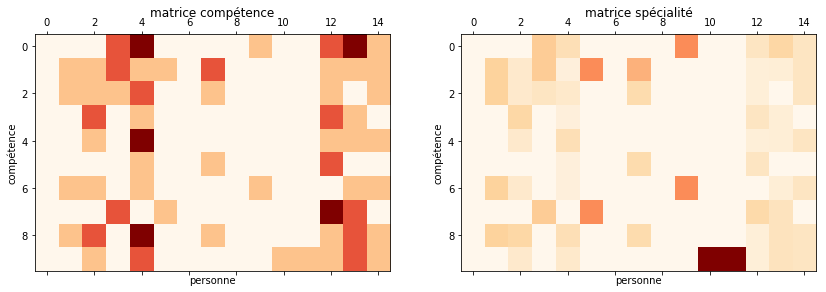
\includegraphics[width=0.99\textwidth]{2matrixassignation}
\end{center}
\end{figure}

La matrice de droite est en fait la matrice de gauche normalisée (L1) en colonne.
Une colonne correspond aux niveaux de compétences d'une personne.\\
Ici par exemple, une tâche relevant de la compétence inscrite à la première ligne devrait être attribuée aux personnes 4 ou 13 (très polyvalentes) selon la première approche, tandis qu'avec la seconde approche cela devrait être la personne 9, plus monovalente.

\paragraph{Heures non assignées :}
il se peut que certaines heures de certaines tâches ne peuvent trouver preneur. Pour modéliser cette situation et garantir l'existence d'une solution mathématique, on pourra assigner une tâche à une personne fictive qui correspondra à une "non assignation". On attribuera à cette action un bénéfice de -100 afin de la pénaliser.





\begin{figure}[H]
\caption{Illustration de la situation}
\begin{center}
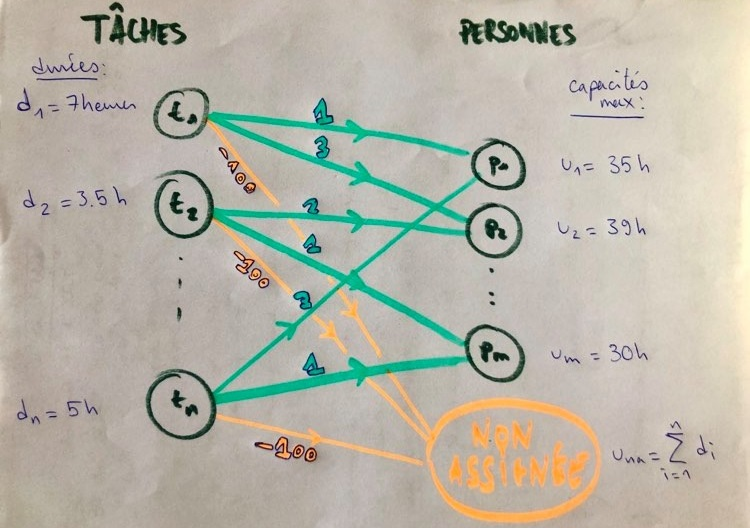
\includegraphics[width=0.75\textwidth]{graphe}
\end{center}
\end{figure}
\newpage



\subsection{Formulation du problème}
On a donc des heures qui doivent partir des tâches pour aller vers les personnes (fictives ou non) en empruntant des arcs plus ou moins avantageux. Egalement, le flot que reçoit chaque personne ne doit pas excéder une certaine quantité.

Notons :
\begin{itemize}
\item $x_{ij}$ le flot sur l'arc $(i,j) \in \mathcal{A}$. Ici l'unité de flot est l'heure.
\item $f_{ij}$ le bénéfice sur l'arc $(i,j) \in \mathcal{A}$.\\
\end{itemize}



On cherche alors à maximiser la quantité suivante :
\[
\sum_{(i,j) \in \mathcal{A}} x_{ij}f_{ij} 
\]

Sous les contraintes :
\[
\underbrace{\forall i = 1,...,n  \sum_{j| (i,j) \in \mathcal{A}} x_{ij} = d_i}_{\text{Distribution de toutes les heures}}
 , \;\;\;
\underbrace{\forall j = 1,...,m  \sum_{i| (i,j) \in \mathcal{A}} x_{ij} \leq u_j}_{\text{Respect des capacités de travail}},\;\;\;
\underbrace{\forall (i,j) \in \mathcal{A},\; x_{ij} \geq 0}_{\text{Positivité}}
\]
Pour mettre le problème sous forme standard c'est à dire uniquement avec des contraintes d'égalités. On doit donc rajouter $m$ variables d'écart. Les contraintes d'inégalités se ré-écrivent donc de la manière suivante : \\


\[
\forall i = 1,...,m, \;\; y_i + \sum_{i| (i,j) \in \mathcal{A}} x_{ij} = u_j, \; y_i \geq 0. 
\]




On a donc ré-écrit le problème sous la forme suivante :
\begin{equation}
\begin{aligned}
\min -f^{t}x\\
\textrm{s.c.} \; \; & Ax = b\\
              & x \geq 0    \\
\end{aligned}
\end{equation}

avec $x \in \mathbb{R}^{card(\mathcal{A}) + m} $, $A \in\mathbb{R}^{(n+m) \times (card(\mathcal{A}) + m)} $, et $b \in\mathbb{R}^{n+m} $.

\newpage
\subsection{Résolution dans python}
\subsubsection{Exemple - Première approche}
En plus de résoudre simplement le problème d'optimisation, on permet au futur l'utilisateur du logiciel d'apprécier quelques indicateurs concernant la solution fournie par le programme.

\begin{code}
DONNEES :

Charge totale de travail   : 445 h pour 70 tâches avec 15 compétences possibles.
							 (6 h/tâche).
Disponibilités totales     : 526 h réparties sur 16 personnes
							 (32 h/personne).
Approche choisie : 1

SORTIE :

Total heures non assignées : 66.0
Niveau moyen de spécialisation pour une heure travaillée : 0.66 / 3
Niveau moyen de spécialisation général : 0.19 / 3

Niveau moyen de compétence pour une heure travaillée     : 1.25 / 3
Niveau moyen de compétence général : 0.45 / 3

Statut résolution : Optimization terminated successfully.
Méthode de résolution      : simplex
fonction objectif          : 6128.0
MESSAGE : CERTAINES HEURES N'ONT PU ETRE ASSIGNEES. SOUHAITEZ-VOUS CONTINUER 
          AVEC UNE POLITIQUE MOINS RESTRICTIVE ?
\end{code}

\paragraph{Remarques et observations :}
\begin{itemize}
\item 66 heures de travail n'ont pû être assignées, on propose donc à l'utilisateur de les assigner en étant moins restrictif.
\item le niveau de spécialisation est un indicateur que l'on créé grâce à la matrice de spécialisation créée précédemment. Il sera intéressant de voir son évolution dans la simulation suivante lorsque l'on aura choisie la deuxième approche pour la conception de la fonction objectif.
\item avec la solution fournie, une heure de travail sera réalisée au niveau de compétence 1.25 / 3 en moyenne. Cette valeur dépend d'une multitude de facteurs : nature des tâches, disponibilités et compétences des utilisateurs, etc.\\

\end{itemize}




Ces indicateurs permettront par exemple à un chef d'équipe d'apprécier la bonne composition de son équipe.\\
En effet, cela pourra l'aider à se rendre compte de plusieurs choses : la charge de travail est-elle disproportionnée par rapport à mon effectif ? Manquerais-je d'architectes ? Les bonnes personnes sont-elles sur les bons projets ?\\

Tout cela contribuera à une vision d'ensemble de qualité sur la santé de l'entreprise, ce qui est exactement la visée du logiciel Teamber.

\newpage
\subsubsection{Exemple - Seconde approche}
On reprend le problème précédant en choisissant la seconde approche, afin d'observer comment cela affecte la forme de la solution.
\begin{code}
DONNEES :

Charge totale de travail   : 445 h pour 70 tâches avec 15 compétences possibles.
							 (6 h/tâche).
Disponibilités totales     : 526 h réparties sur 16 personnes 
							 (32 h/personne).
Approche choisie : 2

SORTIE :

Total heures non assignées : 66.0
Niveau moyen de spécialisation pour une heure travaillée : 0.72 / 3
Niveau moyen de spécialisation général : 0.19 / 3

Niveau moyen de compétence pour une heure travaillée     : 1.23 / 3
Niveau moyen de compétence général : 0.45 / 3

Statut résolution : Optimization terminated successfully.
Méthode de résolution      : simplex
fonction objectif          : 6327.719999999999
PHASE 2 NECESSAIRE
MESSAGE : CERTAINES HEURES N'ONT PU ETRE ASSIGNEES. SOUHAITEZ-VOUS CONTINUER 
          AVEC UNE POLITIQUE MOINS RESTRICTIVE ?
\end{code}
\hypertarget{ref12}{}
\paragraph{Observations :}
\begin{itemize}
\item par rapport à l'approche précédente, le niveau moyen de spécialisation par heure travaillée a augmenté. Difficile de dire si cela est beaucoup mieux en raison de multitudes des paramètres en jeux, mais cela va dans le bon sens.
\item à l'inverse, et cela était prévisible, le niveau moyen de compétence par heure travaillée a diminué (assez peu).\\
\end{itemize}
\hyperlink{Ref10}{Voir un autre exemple en annexe} \\

\paragraph{Commentaire général :}
toutes les données utilisées pour la résolution de ce problème sont simulées aléatoirement. J'ai tenté de créer des données qui reflèteraient le mieux possible la réalité, par exemple lors de la création d'une matrice de compétence, où certaines personnes étaient très polyvalentes et d'autres beaucoup moins.\\

Néanmoins cet effort de représentativité de la réalité a ses limites. Il sera intéressant d'écouter les retours des futurs utilisateurs de cette fonctionnalité, comme pour toutes les fonctionnalités que j'ai développées lors de ce stage.





\newpage
\section{Troisième mission : suggestion d'emplois du temps}
\subsection{Présentation de la mission}


Le deuxième objectif a été le suivant. La 2ème version de TEAMBER sera organisée de telle manière que l'on connaîtra la charge de travail pour un groupe de collaborateurs donné (une équipe). L'enjeu de cette mission est alors de proposer un sprint au chef d'équipe.\\
Un sprint est une planification très précise des tâches qu'une équipe doit réaliser sur une période courte, généralement une semaine mais pouvant aller jusqu'à la quinzaine de jours. En pratique, de nombreuses entreprises s'organisent déjà en sprint sans le savoir car elles planifient le travail par période d'une ou deux semaines.\\
Mais cette planification peut être fastidieuse (2 à 3h chaque lundi matin pour un chef d'équipe par exemple), c'est la raison pour laquelle être capable de proposer une organisation suffisamment logique de leurs sprint aux utilisateurs constituerait un véritable atout pour la deuxième version du logiciel TEAMBER.

\subsection{Données du problèmes et contraintes}

Le sprint lui-même a une date de début et de fin, ainsi qu'une liste de collaborateurs qu'il implique.

\paragraph{Données dont nous disposons pour chaque collaborateur :} 
\begin{itemize}
\item une liste des tâches à programmer dans la période de sprint donnée ; chaque tâche a un niveau de priorité et une durée. 
\item ses horaires de travail. Exemple :
\begin{figure}[H]
\begin{center}
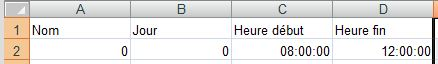
\includegraphics[width=0.50\textwidth]{plagehoraire}
\end{center}
\end{figure}
Ici le collaborateur indique que le lundi matin, il commence à 8h00 et termine à 12h00. Nous appellerons cela une plage horaire d'un collaborateur.

\item les événements déjà planifiés par chacun des collaborateurs sur la période de sprint concernée et qu'ils ne peuvent déplacer, nous les appellerons des "impératifs". Il est préférable pour un collaborateur d'en avoir le moins possible, afin de laisser au mieux le programme construire l'organisation du sprint.

\item sur l'ensemble des tâches de tous les collaborateurs, pourra exister des relations de type mère-fille. Cela pour exprimer que dans certaines situation, Monsieur A doit terminer la tâche X avant que Madame B ne commence la tâche Y. Ces tâches ne représenteront qu'une très faible proportion de toutes les tâches. Nous qualifierons ces tâches de "mère-fille".



\end{itemize}

\medbreak

Il faut aussi penser au fait que les profils des futurs utilisateurs de Teamber pourront être différents : certains préféreront respecter l'ordre des priorités, d'autres tiendront à avoir des emplois du temps les plus remplis possibles. Nous verrons comment nous tiendrons compte de ces préférences dans la section suivante.\\

\hyperlink{ref13}{Voir la librairie rédigée pour la résolution du problème}
\hypertarget{ref14}{}
\newpage
\subsection{Impératifs et tâches mère-fille}
\subsubsection{Prise en compte des impératifs}
Cela constituera la première phase de nos calculs : construire la "base" de l'emploi du temps. Cette base est l'ensemble des plages horaires disponibles restantes à un collaborateur une fois ses horaires et ses impératifs pris en compte. Cette première étape consiste à intersecter chaque impératif avec les plages horaires disponibles de chacun des collaborateurs. 

\subsubsection{Gestion des tâches mère-fille (TMF)}
Dans notre problème, la prise en compte de ces tâches mère-fille (TMF) constitue une contrainte raide, qu'il faut absolument respecter; contrairement aux autres contraintes, plus souples.
\\

Précisément il faut respecter : l'arrangement des tâches, et les disponibilités de chaque utilisateur. De plus, rien n'indique qu'une solution à ce problème existe et il me semble que c'est assez difficile à déterminer rigoureusement.\\

Le problème est alors le suivant : planifier cette suite de tâche dans les emplois du temps des collaborateurs, sans jamais qu'elles ne se chevauchent dans le temps et qu'elles respectent les horaires de travail des collaborateurs auxquels elles sont assignées. La priorité absolue de ce problème est le respect de l'arrangement des tâches, ainsi nous sacrifierons si nécessaire quelques quarts d'heures de présence en plus pour respecter cette contrainte.\\


Nous considèrerons que le temps zéro $t_0 = 0$ est le début du sprint, et que le temps final $t_f$ est la longueur en heures du sprint. Notons également $(t_i)_{i=1,...,n}$ les dates de début (nombres d'heures depuis le début du sprint) des $n$ tâches à planifier, $(d_i)_{i=1,...,n}$ leur durée et $(I_i)_{i=1,...,n}$ la suite de listes de tous les intervalles candidats à contenir chacune des dates de début.

\paragraph{Méthode de résolution :}
\begin{itemize}
\item générer aléatoirement $(t_1,...,t_n)$ suivant la loi des statistiques d'ordre sur $[t_0,t_f]$
\item projeter chaque $t_i$ dans l'intervalle de $I_i$ le plus proche
\item projeter $(t_1,...,t_n)$ dans l'espace vérifiant $t_i + d_i \leq t_{i+1}, \forall i = 1,...,n-1$.
\item calculer un score : le nombre total d'heures séparant les $t_i$ de leur intervalle le plus proche
\item répéter ce procédé 100 fois (par exemple) et garder le meilleur tirage que l'on ait eu.\\
\end{itemize}

Sous réserve que l'utilisateur du logiciel fournisse des données cohérentes : que les disponibilités des utilisateurs,
que la charge de travail qui leur ait attribuée et que la période du sprint soit en phase, alors cette méthode de résolution se montre très efficace et rapide.\\

Ensuite on place ces tâches dans les emplois du temps et on s'attaque à la planification des autres tâches.
\newpage
\subsection{Optimisation d'un emploi du temps avec l'algorithme de recuit simulé}
Avant de déterminer quelle tâche doit être faite à quel moment, on va découper ces tâches en tranches d'une durée maximale choisie par l'utilisateur.\\
Par exemple, une tâche de 3h30 avec une tranche maximale de 1h sera découpée en 3 fois 1h et 1 fois une demi-heure.
Ce découpage offre des avantages :
\begin{itemize}
\item il se peut que certaines tâches aient une durée trop grande (12h par exemple) et ne puisse être casées à aucun endroit de l'emploi du temps.
\item cela permet de mieux remplir l'emploi du temps. En effet, essayer d'arranger des tranches d'1h dans les disponibilités laissera sans doute moins de trous dans l'emploi du temps final que si l'on travaillait avec des durées plus grandes. On perdra donc moins de temps.
\item la sensation de continuité dans le travail sera améliorée. Cette étape permettra de créer des situations réalistes comme : "je commence cette tâche avant manger et je continuerai après manger" ou encore "je terminerai cela demain matin", apportant du naturel dans l'organisation du travail.
\end{itemize}

Le premier inconvénient auquel on s'expose est la dispersion d'une tâche dans le temps. Par dispersion on entend le fait de réaliser une tâche en plusieurs fois, comme la commencer le lundi matin, la reprendre le mercredi et l'achever le vendredi. Ce genre de situation est à éviter, et nous verrons que la plupart du temps nous y parviendrons.\\

Le second inconvénient est l'augmentation du nombre de tâches (comprendre morceaux de tâches désormais) à planifier.\\


Cela dit, il s'agit maintenant de mettre pour un collaborateur, la liste de ses tâches bout à bout, et de regarder la qualité de cet arrangement. Laisse-t-il beaucoup de trous dans l'emploi du temps ? Tient-il suffisamment compte de l'ordre des priorités ? Y a-t-il une bonne continuité comme expliqué précédemment ?\\

Le nombre d'arrangements possibles des tâches étant rapidement trop important, il m'a paru adapté d'utiliser l'algorithme de recuit simulé en définissant une énergie associée à chaque arrangement, pénalisant ceux qui conduisent à de "mauvais" emplois du temps et qui serait minimisée au fur et à mesure des itérations.
\subsubsection{L'algorithme de recuit simulé}
\paragraph{Définition (wikipédia) :} en algorithmique, le recuit simulé est une méthode de programmation empirique (métaheuristique) inspirée d'un processus utilisé en métallurgie. On alterne dans cette dernière des cycles de refroidissement lent et de réchauffage (recuit) qui ont pour effet de minimiser l'énergie du matériau. Cette méthode est transposée en optimisation pour trouver les extrema d'une fonction. Elle a été mise au point par trois chercheurs de la société IBM, S. Kirkpatrick, C.D. Gelatt et M.P. Vecchi en 1983, et indépendamment par V. Černy en 1985. \par



\paragraph{Principe :} partant d'un état initial $x$, et d'une température initiale $T$, on génère à chaque itération un état candidat $y$ voisin de $x$ (on considère que la loi de transition est symétrique). Si cet état candidat a une énergie plus faible que $x$ ($\Delta E < 0$), alors il le remplace; sinon, il le remplace avec probabilité $\exp\left(\frac{-\Delta E}{T} \right)$. A la fin, de cette itération, on fait décroître la température $T$ et si $x$ est le meilleur état que l'on ait rencontré, on le sauvegarde dans une variable $x^{\star}$. On répète cette opération tant qu'une condition d'arrêt n'est pas vérifiée. \par

\paragraph{Pour notre problème :}
\begin{itemize}
\item pour générer un candidat $y$ voisin de $x$, on permutera deux tâches au hasard dans l'arrangement $x$. Cette manière de transiter d'un état à l'un de ses voisins est bien symétrique.
\item notre critère d'arrêt sera un simple nombre d'itérations atteint du type : NOMBRE DE TACHES TOTAL $\times$ 100. 100 est ici arbitraire.
\item on fera décroître la température de manière géométrique jusqu'à atteindre une température minimale à la fin des itérations.
\end{itemize}
\subsubsection{Calcul des énergies}
En notant $a$ l'arrangement des tâches d'un utilisateur et $\lambda$ ses préférences, on calcule l'énergie de cet arrangement :

\[
E (a,p) = \lambda_{p}  V_p(a) + \lambda_{t}  V_{t}(a)  + \lambda_{d} V_{d}(a)
\]

Les fonctions $V$ calculent un potentiel entre 0 et 1 de l'arrangement et les abréviations "p","t" et "d" correspondent respectivement aux non respect des priorités, au temps perdu et au niveau de dispersion qu'engendre l'arrangement $a$.

Les coefficient de pénalisation sont une combinaison convexe, et permettront aux utilisateur d'indiquer leurs préférences.

Il est très important que tous les quantités que l'on manipule soit normalisées (comprises entre 0 et 1). Cela permet de donner lieu à des $\Delta E$ toujours du même ordre quelque soit la configuration, et d'avoir toujours la même gestion de la température.
\paragraph{Calcul du potentiel "Priorités" :} admettons que notre arrangement des taches est tel que le vecteur des priorités est celui-ci : $(5,2,1,3,4,6,4)$. L'arrangement idéal aurait ce vecteur de priorités : $(1,2,3,4,4,5,6)$. On calcule alors la différence en norme $L1$ de ces deux vecteurs, que l'on divise une première fois par le nombre de niveaux de priorités différents (6 ici) puis par le nombre de taches au total (7 ici).

\paragraph{Calcul du potentiel "Temps perdu" :} admettons que les taches aient ces durées en heures $(1.75,0.5,1.25,0.75,2,1.5...)$ et que les plages horaires, aient ces durées: $(4,3.5,2,2...)$. Il s'agit alors de remplir la plage horaire courante tant qu'on le peut, autrement on passe au remplissage de la plage horaire suivante. Une fois une plage remplie, on compte le temps non utilisé de cette plage. On s'arrête une fois que toutes les tâches ont été comptabilisées (on ne compte pas alors le temps restant jusqu'à la fin du sprint comme du temps perdu) ou dès qu'on a épuisé toutes les plages. On retourne alors :
\begin{itemize}
\item un potentiel pour le temps perdu : la somme des temps perdus sur chaque plage horaire utilisée divisée par le temps total disponible sur ces mêmes plages. 
\item un vecteur contenant la correspondance entre l'identifiant de la tâche et l'identifiant de la plage horaire dans laquelle elle tombe.
\end{itemize}


\paragraph{Calcul du potentiel "Dispersion" :} considérons une tâche de 3h30 qui peut être réalisée en au maximum 4 fois (3 * 1h + 1*0.5h). Si elle est réalisée en 4 fois, alors son taux de dispersion est de 100\%, en 3 fois : 66\%, 2 fois : 33\% et 1 fois : 0\%. On fait la moyenne de ces taux de dispersion pour les tâches qui peuvent être réalisées en plusieurs fois. On considère ici qu'une interruption est simplement le fait de se consacrer à une autre tâche avant de reprendre la première, ainsi le fait de reprendre une tâche après manger, le lendemain en revenant au travail, ou après un impératif ne constitue pas une interruption.
 





\newpage
\subsection{Simulation - Planification de tâches mère-fille}

Dans cet exemple, tous les utilisateurs travaillent de 8h à 12h et de 13h à 17h chaque jour de la semaine. Ils ont tous les mêmes impératifs que l'on peut apercevoir plus bas.

Dans un premier temps, on indique l'équipe à concernée par les tâches que l'on souhaite affecter et les tâches elle même.

Dès lors l'utilisateur n'intervient plus dans le programme.

\begin{figure}[H]
\begin{center}
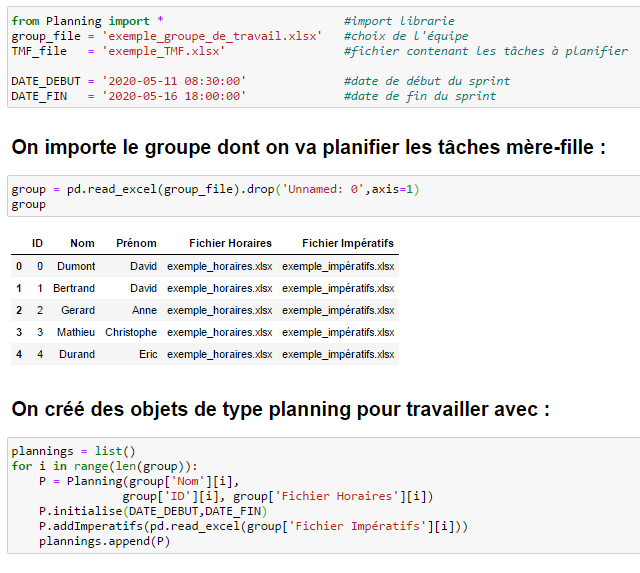
\includegraphics[width=0.99\textwidth]{tmu1}
\end{center}
\end{figure}





\begin{figure}[H]
\begin{center}
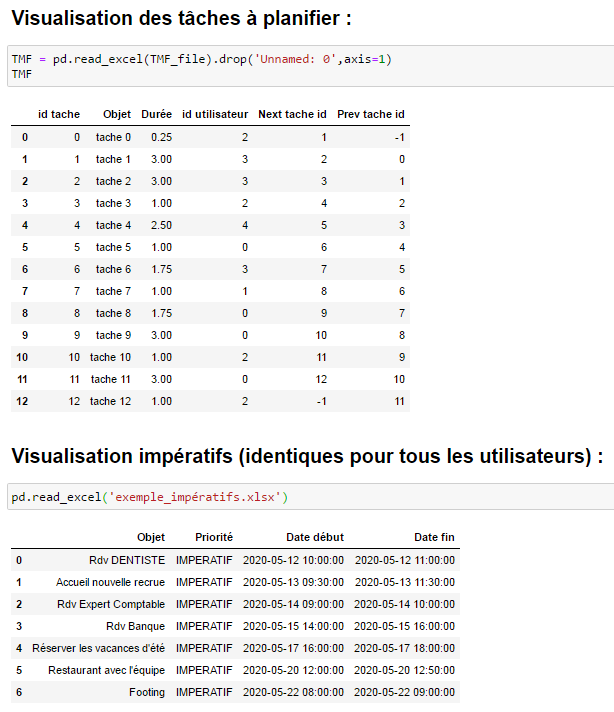
\includegraphics[width=0.95\textwidth]{tmu2}
\end{center}
\end{figure}

On observe que la meilleure solution que l'on ait trouvé retire une heure de temps libre au total au groupe de travail pour de réussir à planifier ces tâches.\\

Enfin on peut constater que les tâches ont bien été placées dans les emplois du temps.


\newpage
\begin{figure}[H]
\begin{center}
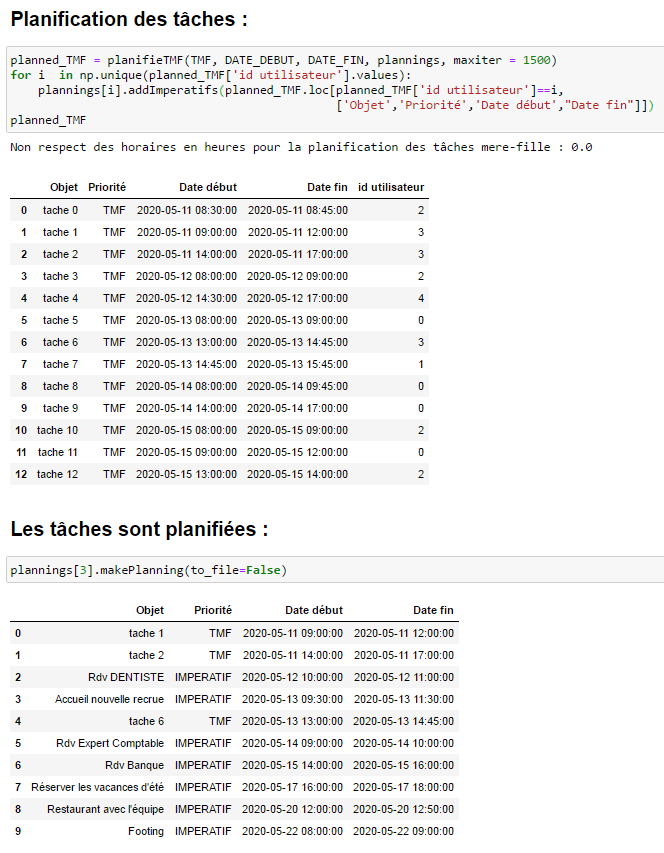
\includegraphics[width=0.99\textwidth]{tmu3}
\end{center}
\end{figure}

Ci-dessus l'emploi du temps l'utilisateur n°3.

On voit qu'on a trouvé une solution respectant toutes les contraintes. 

\newpage
\subsection{Simulations - Optimisation d'un emploi du temps}

D'abord on créé un objet planning auquel on ajoute tous les paramètres de la planification :

\begin{code}
P = Planning(nom_utilisateur=nom_utilisateur,
        id_utilisateur=id_utilisateur,
        plagehoraire_filename=plagehoraire_filename)

t = pd.read_excel(tasks_filename)
tasks = split_tasks(t,1)#.reset_index(drop=True)
P.addTasks(tasks)
P.initialise(DATE_DEBUT,DATE_FIN)
P.addImperatifs(pd.read_excel(imperatifs_filename))
\end{code}

Ensuite on peut changer les préférences (qui se normalisent automatiquement) lors de l'optimisation :
\begin{code}
P.setPenalties([1,4,1])
\end{code}
\begin{verbatim}
OUTPUT :
array([0.16666667, 0.66666667, 0.16666667])
\end{verbatim}

On peut à présent lancer l'optimisation :
\begin{code}
P.Optimise(show=True)
\end{code}


\begin{figure}[H]
\begin{center}
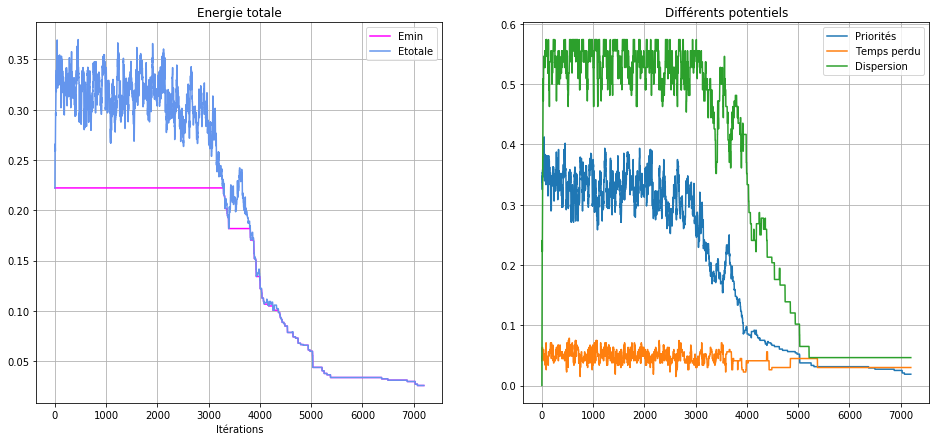
\includegraphics[width=0.99\textwidth]{oedt1}
\end{center}
\end{figure}

On voit que l'on arrive à minimiser toutes les composantes de notre critère.

Page suivante, obeservons l'emploi du temps résultant de cette optimisation.

\newpage	
Les horaires sont 8h-12h et 13h-17h tous les jours de la semaine; la période de planification des tâches commence le 11 mai 2020 8h30 et se termine le 15 mai 2020 18h00.
\begin{figure}[H]
\begin{center}
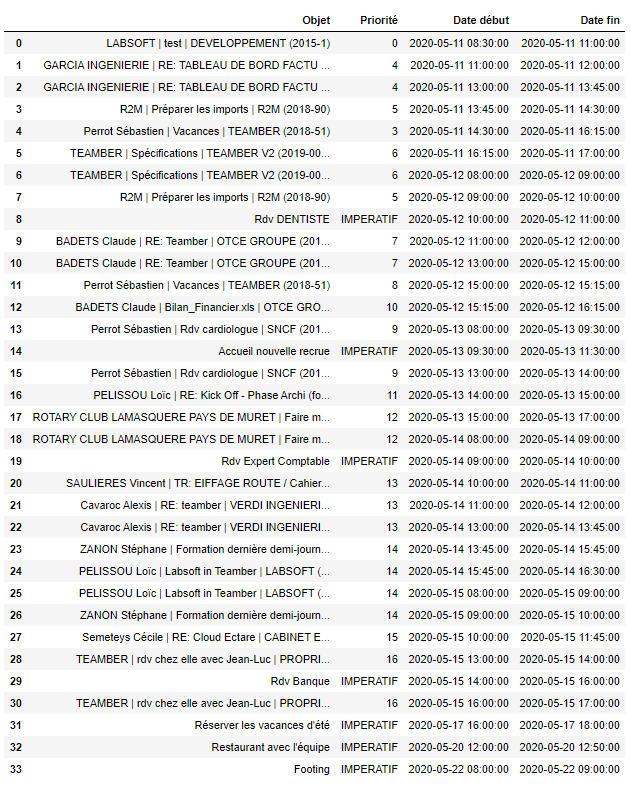
\includegraphics[width=0.99\textwidth]{oedt2}
\end{center}
\end{figure}

\newpage
\paragraph{Rermarques :}
\begin{itemize}
\item si certaines tâches durent plus d'une heure alors qu'elles ont été découpées en tranche d'une heure maximum, c'est parce qu'on les a recollées lorsque cela était possible. Cela offre une meilleure lisibilité.
\item les tâches sont quasiment classées par ordre de priorité, hormis ligne 12-13 ou cela a permis de caser une tâche d'1h30 dans un créneau d'exactement 1h30, idéal !
\item les calculs ont pris environ de 5 secondes au total, ce qui est raisonnable.
\item les tâches sont quasiment toujours réalisées en une fois.\\
\end{itemize}

Observons à présent les tâches qui n'ont pu être planifiées :

\begin{figure}[H]
\begin{center}
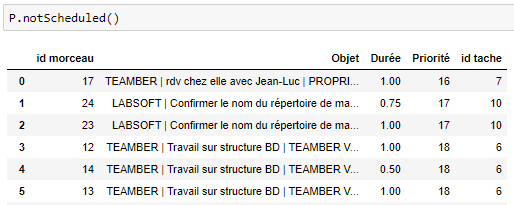
\includegraphics[width=0.85\textwidth]{oedt3}
\end{center}
\end{figure}

En ayant connaissance de cette information, un chef d'équipe pourra donc choisir de relancer les calculs en changeant les horaires des membres de son équipe afin d'atteindre les objectifs dans les temps impartis.

\subsection{Conclusion}

L'outil créé arrive à générer en des temps raisonnables des emplois du temps respectant dans l'ensemble plutôt bien les contraintes décrites en introduction du problème. Pour rappel, il s'agit plus de suggérer que d'imposer les emplois du temps aux utilisateurs, libre ensuite à eux d'appliquer des corrections. Pour la deuxième version du logiciel Teamber, cet outil offrira, on l'espère plusieurs avantages :
\begin{itemize}
\item aider un chef de projet dans la planification de la semaine pour son équipe en accomplissant le gros du travail. Pour la prochaine version du logiciel Teamber, s'agissant de ce module de planification, on imagine que l'utilisateur pourra lancer plusieurs fois les calculs en jouant sur les paramètres et retenir la proposition de sprint qui lui conviendra le mieux.

\item une utilisation personnelle sur du très court terme : un utilisateur qui n'a pas réussi à terminer tout ce qu'il s'était planifié dans la journée, cliquerait à ce moment là sur un bouton "Replanifier les tâches inachevées" et le programme lui ré-organiserait son emploi du temps à partir du lendemain.\\
A l'inverse, si à un certain moment l'utilisateur est avance dans son travail, il pourra reprogrammer son emploi du temps à partir de cet instant.

\item des agendas lisibles pour tous les utilisateurs. L'idée étant d'éviter à tout prix les agendas qui renvoient une sentiment de débordement, dans lesquels les événements se chevauchent, témoignant d'un travail dans l'urgence souvent peu efficace.

\item contribuer à une meilleure organisation de l'entreprise, le leitmotiv du logiciel Teamber.
\end{itemize}












\newpage
\section{Quatrième mission : complétion intelligente d'une tournée commerciale}
L'idée est la suivante : un commercial dispose d'une succession de rendez-vous datés et localisés pour sa tournée. Il va donc faire un certain nombre de trajets. \\
D'autre part, existera dans la seconde version de TEAMBER une liste de \textbf{clients} et une liste de \textbf{prospects}. Seront renseignés dans ces listes la date de dernière visite, et pour les prospects, une espérance de concrétisation allant de zéro à cent pourcents. \\
Au moment d'utiliser le logiciel pour compléter sa tournée, l'utilisateur indiquera une sélection de lieux qu'il accepte d'éventuellement ajouter à sa tournée initiale. Trois sélections seront possibles : 
\begin{itemize}
\item Sélection 1 : prospects tels que Date dernière visite > 3 mois et espérance concrétisation > 70\%
\item Sélection 2 : prospects tels que Date dernière visite > 3 mois
\item Sélection 3 : prospects et clients tels que Date dernière visite > 4 mois.
\end{itemize}
A noter que rien n'empêche de personnaliser davantage la sélection, mais c'est ce qui m'a été demandé pour ce programme.

\subsection{Données et contraintes du problème}
\paragraph{Données :}
Sur la base de la tournée initiale du commercial (voir Figure 4) on va tâcher d'ajouter intelligemment et dans la mesure du possible des points de passage sur sa route.


\begin{figure}[H]
\caption{Exemple de tournée initiale}
\begin{center}
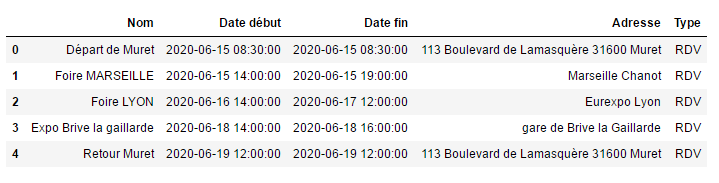
\includegraphics[width=0.90\textwidth]{dfrdv}
\end{center}
\end{figure}


\paragraph{Contraintes :}
\begin{itemize}
\item on doit fournir une charge de travail cohérente au commercial, pour cela il pourra indiquer qu'il est disponible de telle heure à telle heure chaque jour.
\item il s'agit de le faire dévier le moins possible de son itinéraire initial afin de minimiser le temps de trajet.
\item selon qu'on aille visiter un prospect ou un client, le temps passé sur place varie, on pourra indiquer des temps référents selon la catégorie de l'endroit visité. On considèrera dans notre cas qu'on accorde en moyenne 2h à un client et 30min à un prospect.
\item notre programme doit être simple d'utilisation, le plus rapide possible, et son utilisation la moins coûteuse possible (frais Google maps).
\end{itemize}

\subsection{Méthode de résolution}

Assez simplement, entre chaque paire de rendez-vous, on va ajouter des visites tant que faire se peut.\\
A l'aide des horaires de référence du commercial et ceux des deux rendez-vous consécutifs, on a alors une idée du temps restant disponible dont il dispose entre les deux rendez-vous, on va alors chercher la meilleure visite possible.\\

La meilleure visite possible doit être réalisable (temps passé sur place + temps déviation trajet < temps restant disponible) et telle que le temps de déviation est minimal. S'il y a une visite candidate, alors on l'ajoutera à notre tournée, et on actualisera le temps restant disponible et l'on cherchera une nouvelle candidate.\\

L'utilisateur indiquera également une durée qui correspondra à une marge de sécurité (1h par exemple). Une fois que le temps restant disponible tombera en dessous de ce seuil, l'on s'arrêtera d'ajouter des points d'arrêts sur le trajet.\\

\subsubsection{Raffinage géographique de la sélection}
Afin de mettre en place ce programme, il est nécessaire de connaître les durées de trajet (Distance Matrix) entre toutes les adresses postales impliquées dans ce programme. Cela se fait au travers de google maps developper à l'aide d'une clé API.\\

Ce service est payant, j'ai pu utiliser la période d'essai pour mettre en place le programme.\\
Les calculs prennent un certain temps, (N adresses donnent N² calculs d'itinéraires), et le coût étant proportionnel aux nombre de demandes effectuées, il faut donc ne garder dans notre sélection d'adresses candidates des adresses qui sont cohérentes vis à vis de notre tournée.\\

Dans un premier temps, j'avais pensé à inviter l'utilisateur à préciser les régions/départements concernés par sa tournée pour filtrer les adresses par leur code postal. Mais cela contribuerait à la pénibilité d'utilisation du programme.\\

Des adresses cohérentes sont en réalités des adresses qui ne nous font pas tellement dévier l'itinéraire original : celui qui mène de rendez-vous ferme en rendez-vous ferme. Ainsi il faut réussir à attraper les adresses se situant suffisamment proche de cet itinéraire.\\

Pour cela, en utilisant le module "Directions" de la google maps API, on va pouvoir obtenir une succession de points (latitude-longitude) pour un trajet donné. Ces points correspondent à des instructions GPS (tourner à gauche, prendre la sortie 37 etc. ).

A partir de ces points, on va pouvoir dessiner des cercles d'un rayon fixé en préambule du programme et ne conserver que les adresses tombant dans au moins un de ces cercles.


En vert : les adresses retenues, en noir : les adresses écartées, en rouge : les étapes de notre itinéraire initial.
\newpage
\begin{figure}[H]
\begin{center}
\caption{Raffinage géographique de la sélection}
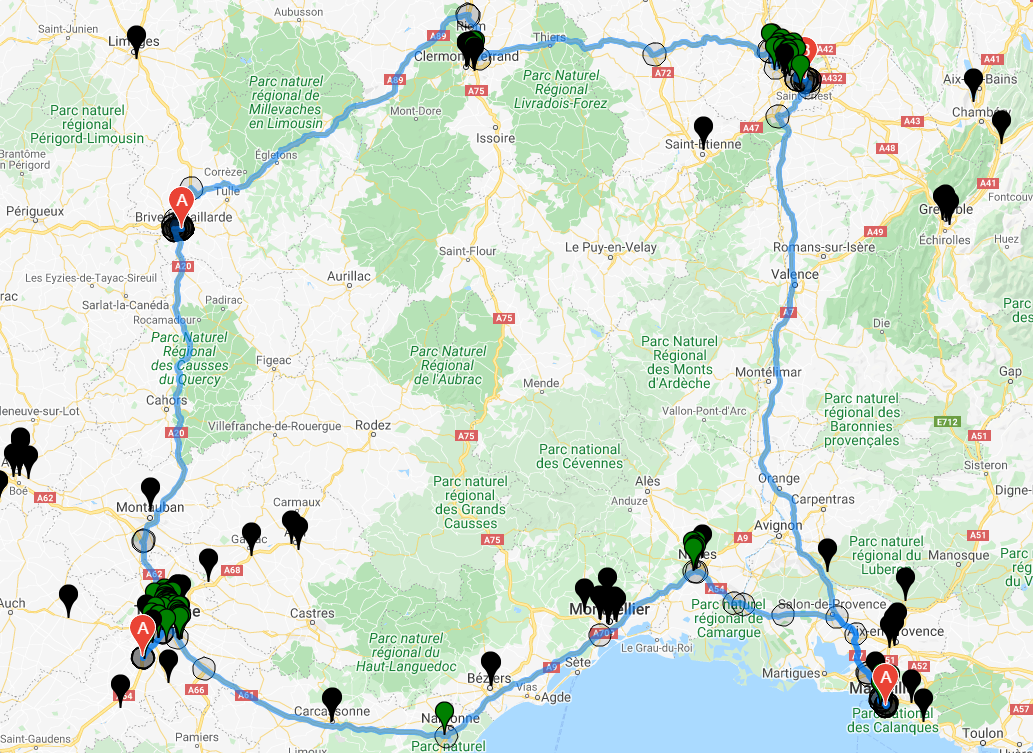
\includegraphics[width=0.85\textwidth]{Circles2}
\end{center}
\end{figure}



\paragraph{Remarques :}
\begin{itemize}
\item les cercles étant centrés sur des intersections, des bifurcations ou autre nous empêche parfois de capter les adresses à proximité des autoroutes (voire Carcassone).
\item ce filtrage nous a permis de passer de 326 adresses à 86 pour cet exemple.
\end{itemize}  



\begin{figure}[H]
\caption{Distance Matrix et Duration Matrix }
\begin{center}
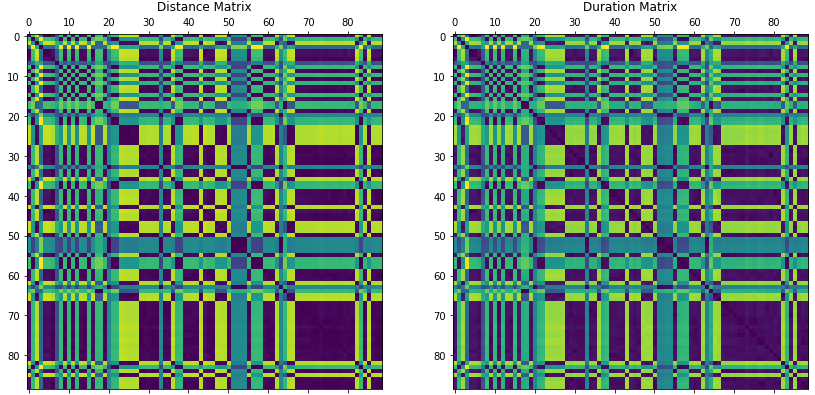
\includegraphics[width=0.82\textwidth]{distance matrix}
\end{center}
\end{figure}

\newpage

\subsubsection{Résultats}

\begin{verbatim}
Import librairies
Import contacts
Sélection
Mode sélection : 1
	88 adresses candidates
Obtention de points le long de la route 
Raffinage des adresses grâce aux cercles 
	Avant raffinage : 326
	Après raffinage : 86
	pour des rayons de : 5000 m.
Obtention de la distance/duration matrix
Optimisation de la tournée
Calcul des horaires de passages pour la tournée
Temps total : 22.08952021598816
Dessin de la tournée
\end{verbatim}

\begin{figure}[H]
\caption{Résultat}
\begin{center}
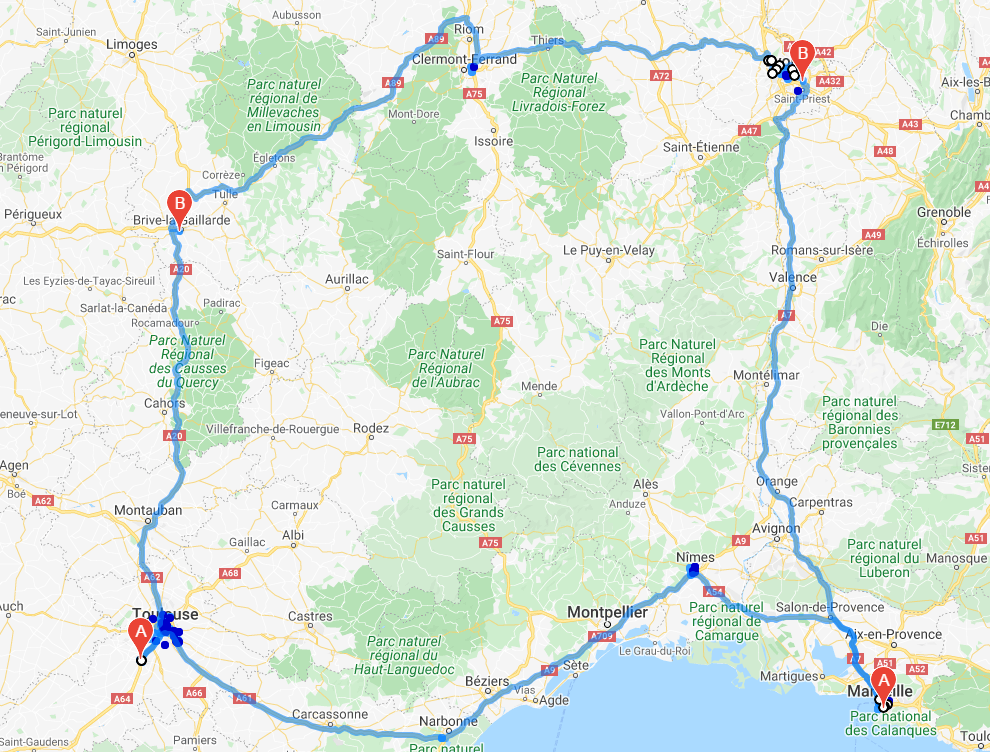
\includegraphics[width=0.95\textwidth]{completion final}
\end{center}
\end{figure}

En bleu clair : les prospects, en bleu foncé : les clients, et en noir et blanc : les étapes ajoutées à la tournée initiale.
\hyperlink{Ref5}{Voir le zoom de la carte}
\hypertarget{Ref6}{}

\newpage


On peut ensuite établir un planning de la tournée, afin de connaître les horaires de passages dans les étapes ajoutées et être en mesure de prévenir les intéressés de notre prochain passage.

\begin{figure}[H]
\caption{Résultat}
\begin{center}
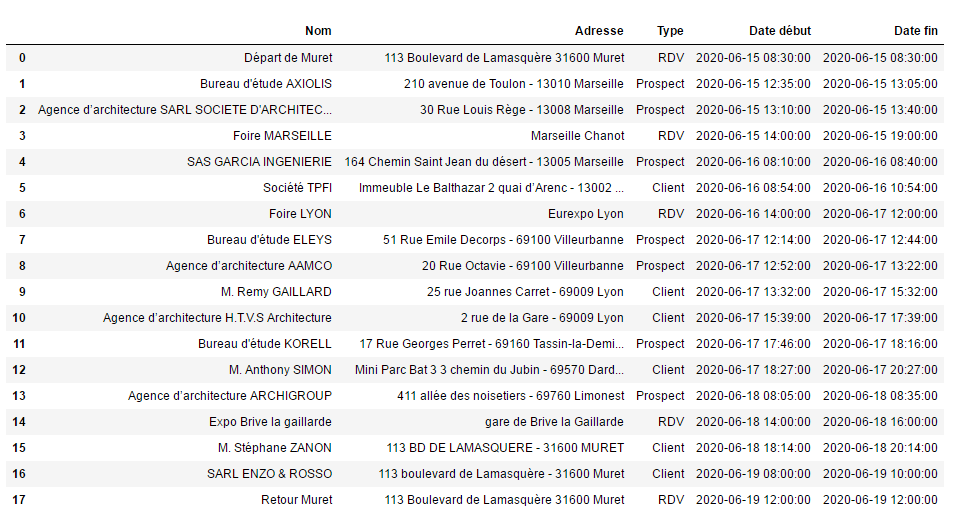
\includegraphics[width=0.95\textwidth]{completion programme}
\end{center}
\end{figure}


\begin{figure}[H]
\caption{Détail des étapes ajoutés entre les RDV}
\begin{center}
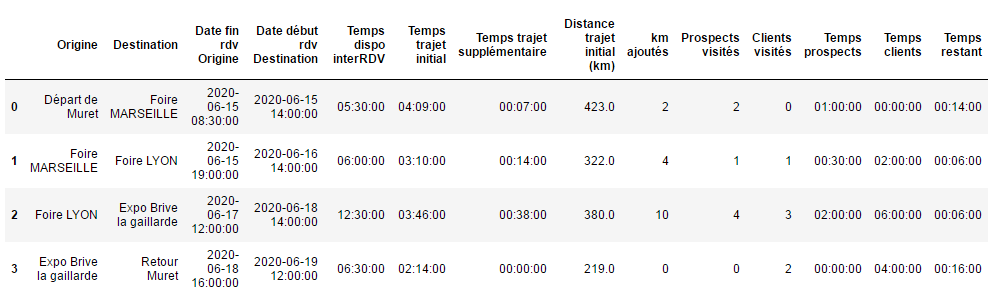
\includegraphics[width=0.95\textwidth]{interrdv}
\end{center}
\end{figure}




\newpage
\section{Cinquième mission : programmation d'une tournée optimale}
Dans cette section, nous devons résoudre le problème du voyageur de commerce.
Il consiste en trouver le plus court trajet reliant un point de départ, des adresses de clients fournies par l'utilisateur et un point d'arrivée.

Ces adresses doivent pouvoir être choisies de différentes manières :
\begin{itemize}
\item une liste explicite fournie par l'utilisateur.
\item en filtrant par région/département les clients recensés dans la base de données TEAMBER.
\item en choisissant l'ensemble des clients contenus dans un cercle de rayon et de centre donnés.
\end{itemize}

Une fois les adresses connues, il s'agira alors de déterminer un trajet optimal ou quasi-optimal.\\

Nous verrons dans la sous-section suivante que des difficultés nous conduiront à trouver une alternative à l'algorithme du recuit simulé, qui ne fonctionne pas parfaitement dans un certain nombre de situations.

\subsection{Trajet optimal - Recuit simulé}

\begin{figure}[H]
\caption{Adresses à Toulouse}
\begin{center}
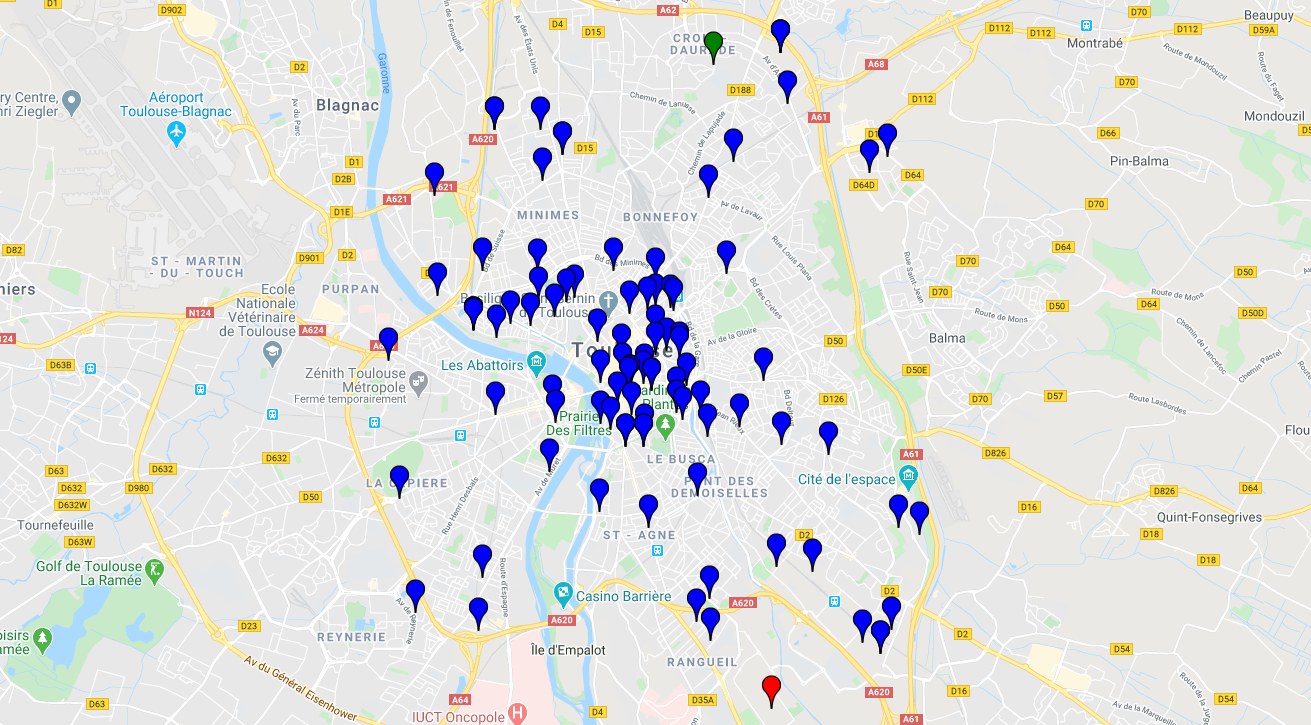
\includegraphics[width=0.95\textwidth]{adresses toulouse}
\end{center}
\end{figure}
\paragraph{Remarques :}
\begin{itemize}
\item dans l'algorithme de recuit simulé, on considèrera qu'un état voisin $y$ de l'état $x$ est tel que l'on peut passer de $x$ à $y$ en retournant une chaîne d'adresses dans $x$. Cette manière de transiter d'un état à l'autre est symétrique.
\item dans ces exemples on considèrera la distance à vol d'oiseau entre les adresses, afin d'économiser des crédits google maps et de s'assurer visuellement de la qualité des résultats.
\item d'autres modes de déplacement seront disponibles : en voiture, à pied, en vélo, en transports.
\end{itemize}
\newpage




\begin{figure}[H]
\caption{Solution après recuit simulé}
\begin{center}
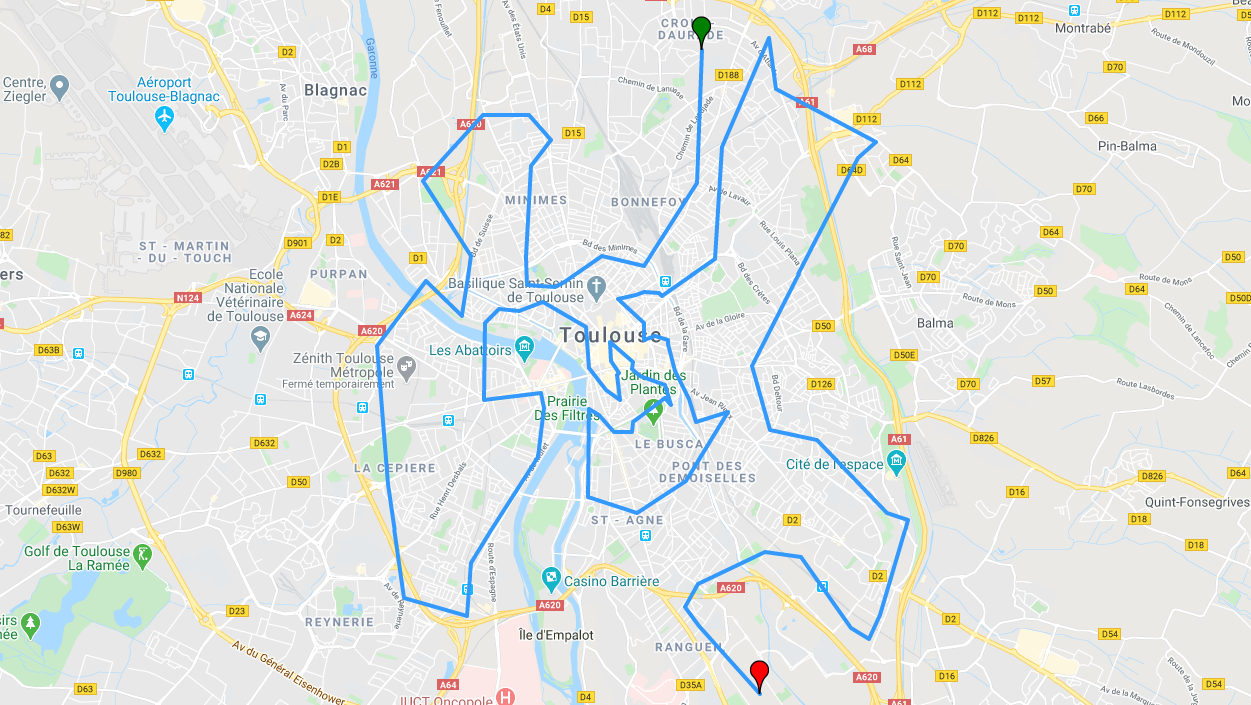
\includegraphics[width=0.95\textwidth]{toulouse tournee opti}
\end{center}
\end{figure}
\hypertarget{Ref8}{}
La solution est satisfaisante. \hyperlink{Ref7}{Voir trajet optimal dans Toulouse à pied}
\subsubsection{Limites}
A présent, un deuxième exemple qui va mettre en difficulté notre méthode de résolution :

\begin{figure}[H]
\caption{Tournée région Rhônes-Alpes}
\begin{center}
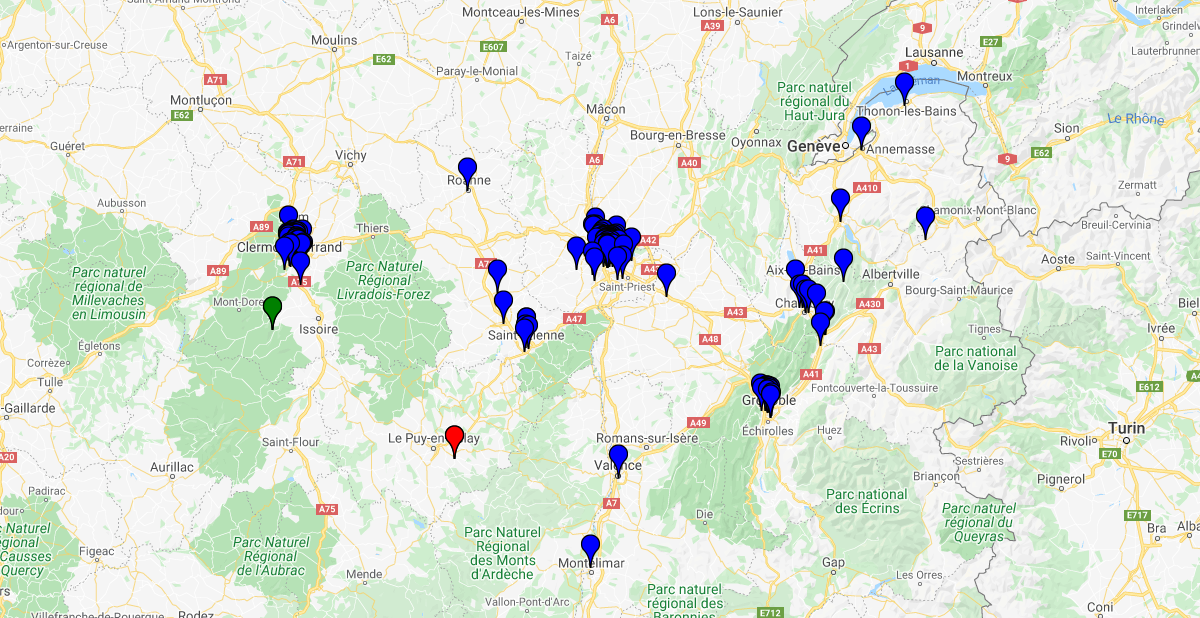
\includegraphics[width=0.95\textwidth]{adresses ra}
\end{center}
\end{figure}

\newpage

\begin{figure}[H]
\caption{Solution recuit simulé - Rhônes-Alpes}
\begin{center}
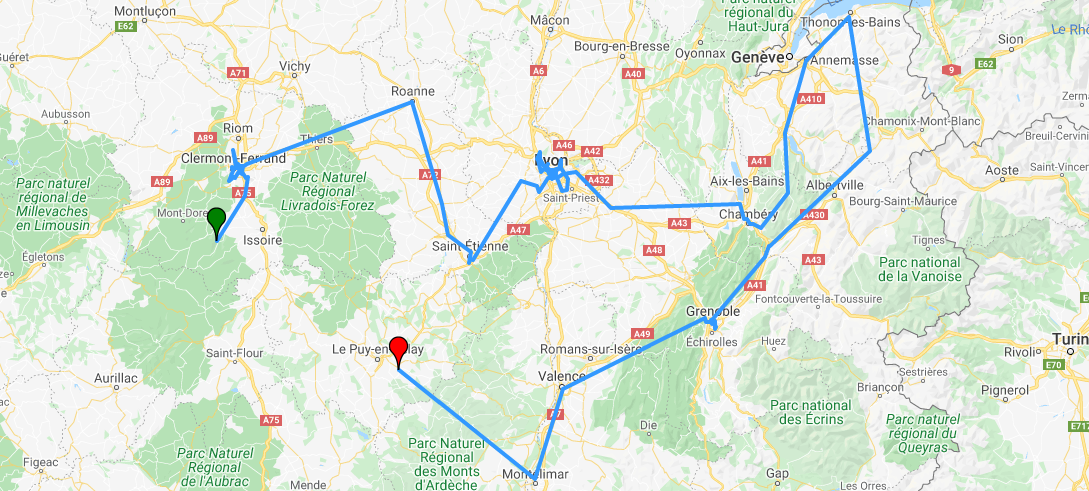
\includegraphics[width=0.98\textwidth]{ra erreur1}
\end{center}
\end{figure}

De loin, le trajet est cohérent, mais à l'intérieur des villes, les trajets ne sont pas optimaux.

\begin{figure}[H]
\caption{Erreurs dans les villes}
\begin{center}
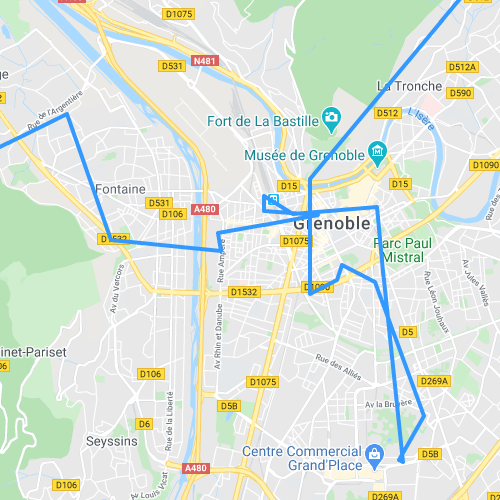
\includegraphics[width=0.49\textwidth]{ra erreur 2}
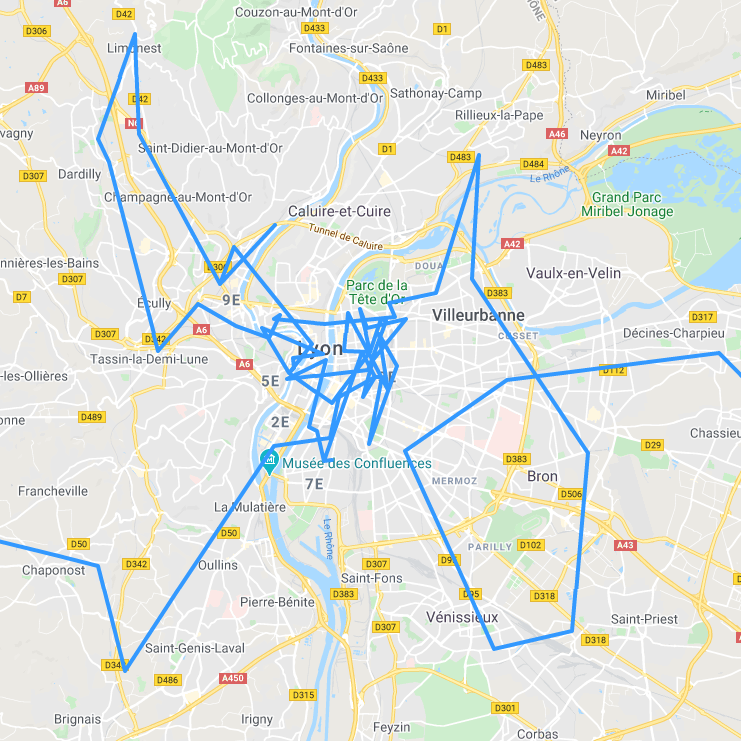
\includegraphics[width=0.49\textwidth]{ra erreur 3}
\end{center}
\end{figure}

Cela vient du fait que les distances entre les adresses à l'intérieur des villes sont négligeables devant d'autres distances. Les distances ne sont pas suffisamment homogènes.

Nous remédions à ce problème dans la section suivante.

\newpage
\subsection{Clustering d'adresses}


Afin de remédier au problème rencontré dans la section précédente, on choisi de regrouper les adresses dans des clusters.


\begin{figure}[H]
\caption{151 adresses  dans la région Auvergne Rhônes-Alpes}
\begin{center}
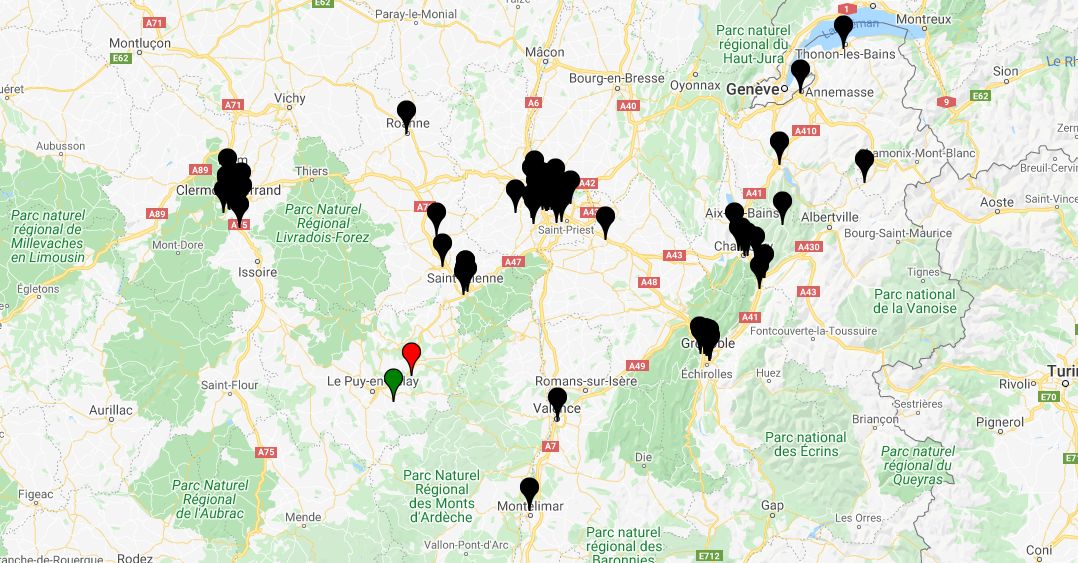
\includegraphics[width=0.98\textwidth]{capture_adresses}
\end{center}
\end{figure}


Nous utiliserons l'algorithme des k-moyennes afin d'identifier formellement des clusters dans cet ensemble de positions géographiques.


\begin{figure}[H]
\caption{Clustering avec k-means}
\begin{center}
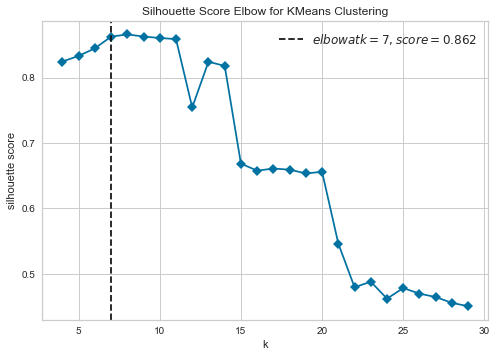
\includegraphics[width=0.49\textwidth]{kmeans-silhouette}
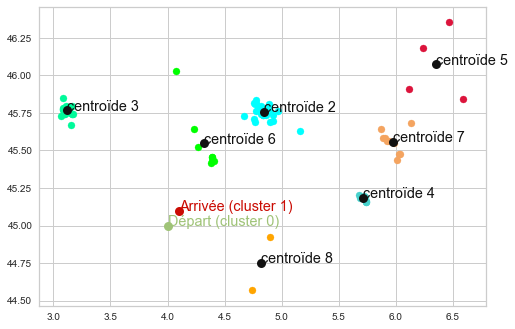
\includegraphics[width=0.49\textwidth]{kmeans-clustering}
\end{center}
\end{figure}

On s'appuie sur l'indice de Silhouette afin de déterminer un nombre de cluster optimal. On peut donc fournir une suggestion de regroupement d'adresses à l'utilisateur.
\newpage
\paragraph{Remarques :}
\begin{itemize}
\item si le nombre de clusters paraît incohérent, l'utilisateur peut toujours le modifier.
\item on considère (de force) que les adresses de départ et d'arrivée comme deux clusters d'une seule adresse. Cela rajoute augmente donc le nombre de cluster de 2.\\
\end{itemize}


Une fois que l'on a déterminé les clusters, nous allons déterminer un ordre de passage optimal dans ces clusters à l'aide des coordonnées GPS des centroïdes.

\begin{figure}[H]
\caption{Ordre de passage optimal dans les clusters et distance matrix}
\begin{center}
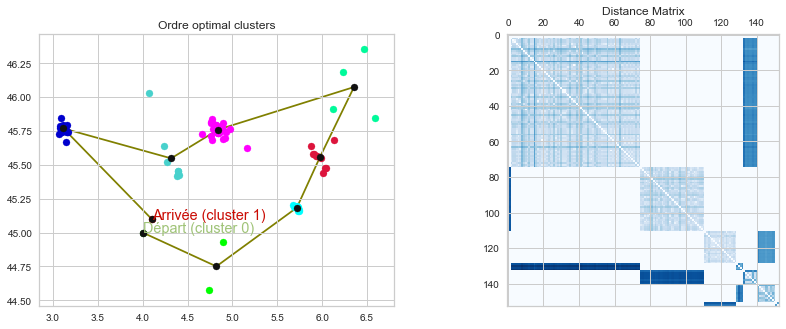
\includegraphics[width=0.99\textwidth]{ARA_ordre_clusters_distance_matrix}
\end{center}
\end{figure}

\paragraph{Remarque} Nous n'avons besoin que des distances sein des clusters eux-mêmes et d'un cluster au suivant (voir Figure 13 graphe de droite). Ici par exemple on fera 8625 requêtes d'itinéraires à Google maps API en fonctionnant par clusters au lieu de 22801 sinon.\\ 




\paragraph{Entrées et sorties des clusters :} nous allons maintenant déterminer des adresses de sortie et d'entrée pour chacun de ces clusters. Pour les paires de clusters successifs, nous allons devoir trouver la meilleure sortie et la meilleure entrée. Si possible, (c'est à dire que le cluster contient au moins deux adresses) nous ne passerons pas deux fois par la même adresse.\\
Encore une fois nous utiliserons le recuit simulé pour résoudre ce problème : étant donnée une liste d'entrées/sorties pour chacun des clusters, nous choisirons un cluster aléatoirement selon son poids (son nombre d'adresses par rapport au nombre d'adresses total) et changerons aléatoirement (une chance sur deux) son entrée ou sa sortie par une adresse qui n'est pas utilisée si possible. Sinon : pour 2 adresses, échange entrée/sortie, sinon pour 1 adresse : rien. Cette manière de procéder est bien symétrique d'une configuration à la configuration voisine.\\
Nous tentons alors de minimiser la somme des distances d'une sortie à l'entrée suivante.

\begin{figure}[H]
\caption{Calcul des entrées/sorties optimales des clusters}
\begin{center}
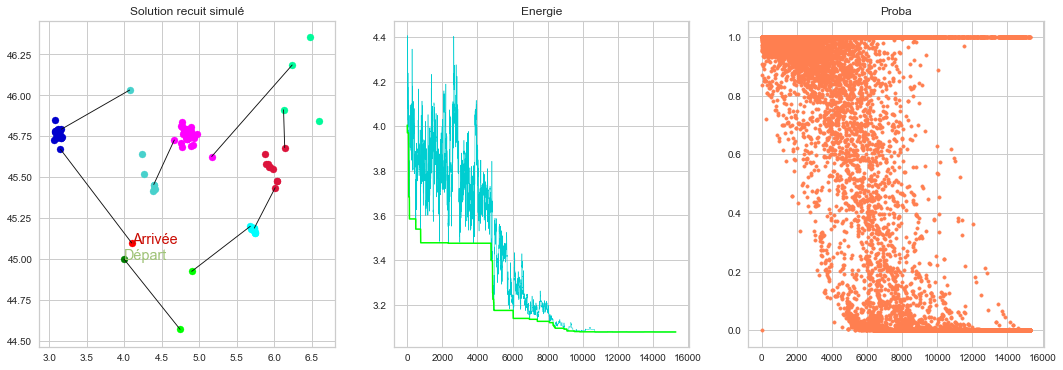
\includegraphics[width=0.99\textwidth]{ARA_entrees_sorties}
\end{center}
\end{figure}


A présent il ne reste plus qu'à déterminer les trajet optimaux  au sein de chaque cluster entre l'entrée et la sortie (recuit simulé), et à mettre tous les trajets bout à bout.

\begin{figure}[H]
\caption{Trajet final}
\begin{center}
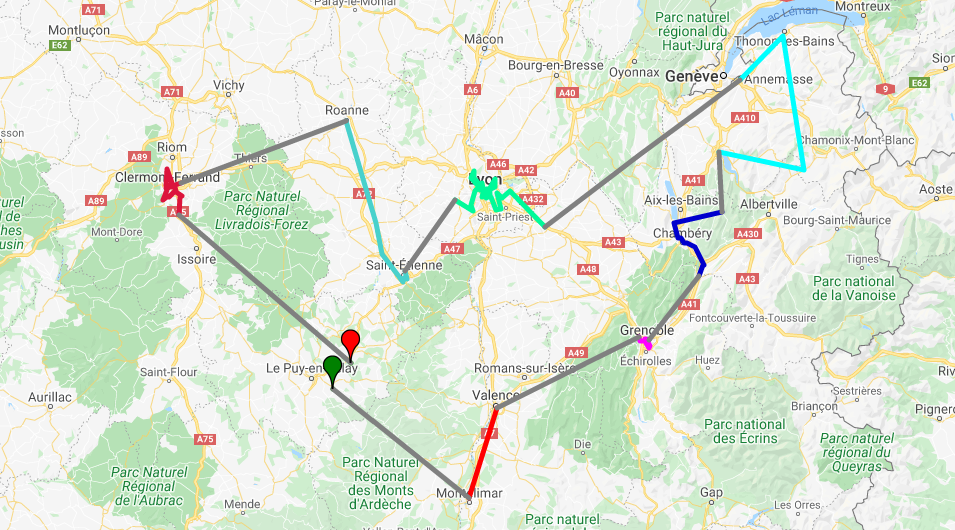
\includegraphics[width=0.99\textwidth]{kmeans-final}
\end{center}
\end{figure}

\newpage
\begin{figure}[H]
\caption{Zoom sur les clusters importants}
\begin{center}
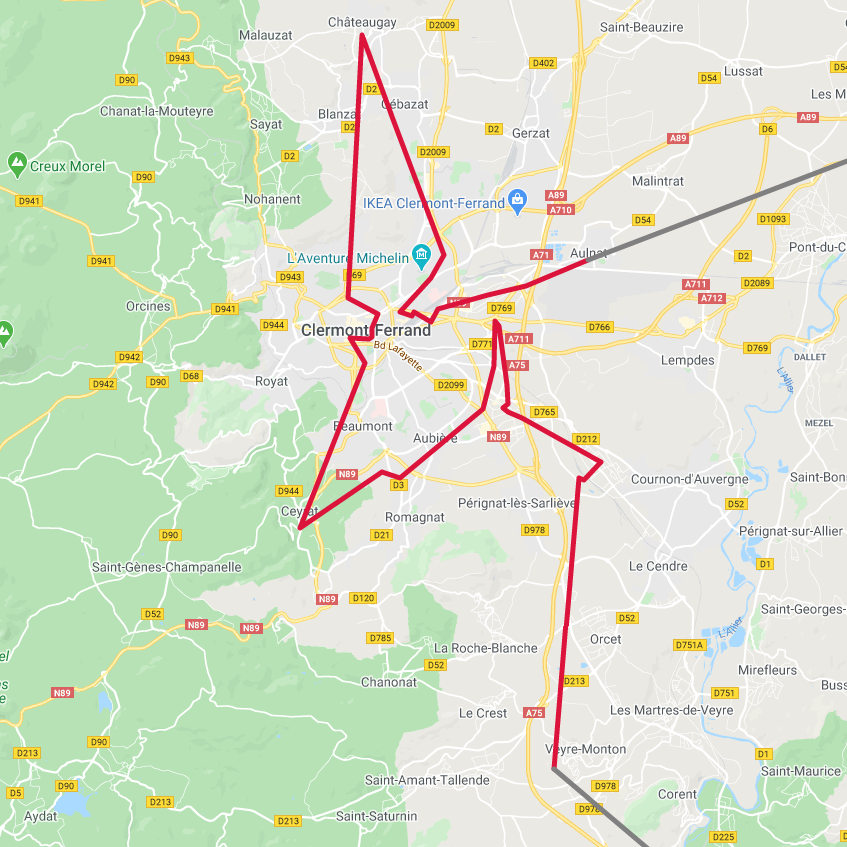
\includegraphics[width=0.32\textwidth]{erreur1}
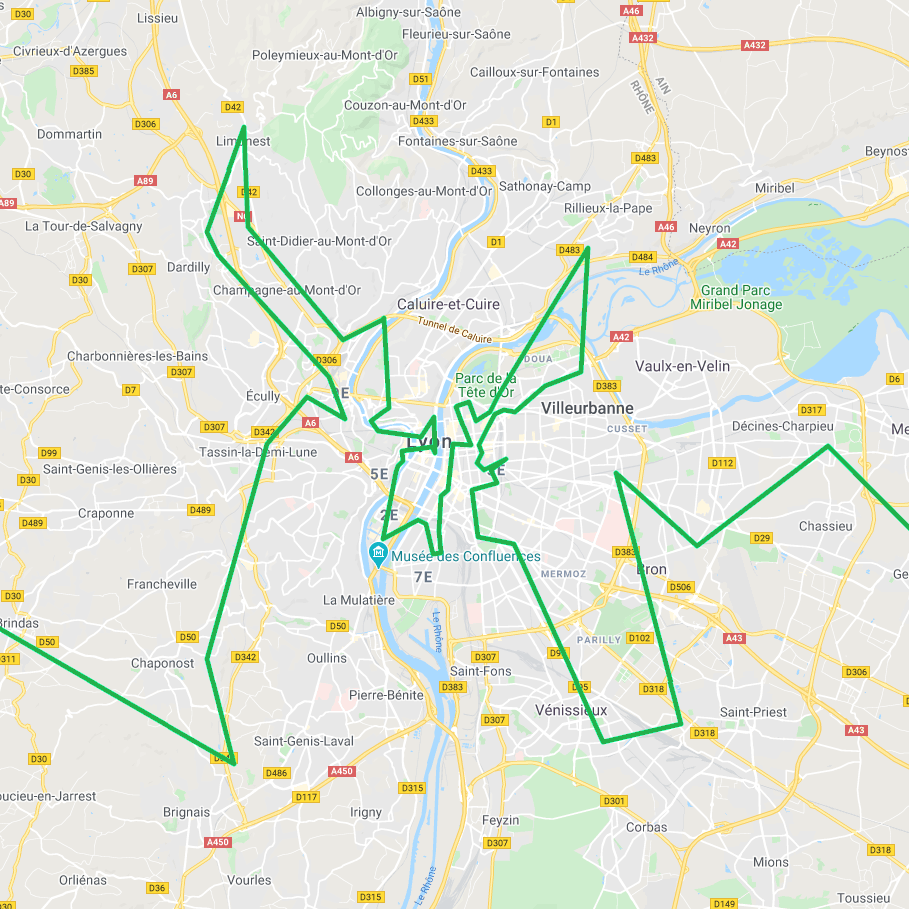
\includegraphics[width=0.32\textwidth]{erreur2}
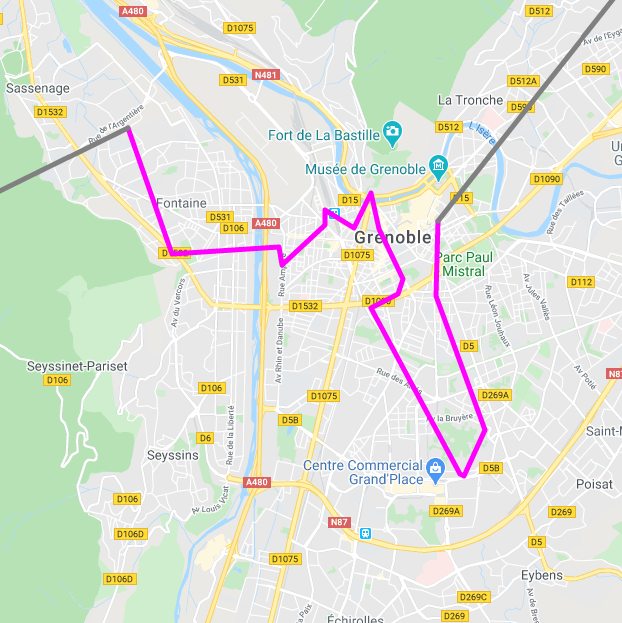
\includegraphics[width=0.32\textwidth]{erreur3}
\end{center}
\end{figure}



\paragraph{Quelques observations :}
\begin{itemize}

\item Nous avons ici optimisé la distance à vol d'oiseau entre nos adresses afin de nous assurer visuellement du bon fonctionnement du programme. Mais par la suite, au sein des clusters ainsi que d'un cluster au suivant, l'utilisateur choisira d'optimiser le temps de trajet (ce qui sera sans doute le cas la plupart du temps) ou le nombre de km parcourus.

\item Il sera également possible de déterminer la zone de tournée commerciale en indiquant un centre et un rayon, ainsi on cherchera le meilleur trajet entre les adresses de ce disque. C'est même la plupart du temps que cela fonctionnera. De ce fait, connaître les coordonnées GPS des adresses est indispensable.

\item D'autres exemple d'optimisations de tournées sont visibles en \hyperlink{Ref1}{annexe} (toujours avec la distance à vol d'oiseau). 

\item \hypertarget{Ref2}{Lorsque} nous cherchons un ordre de passage entre les clusters, nous faisons l'hypothèse que la distance à vol d'oiseau et temps de trajet sont  suffisamment corrélées. Cette hypothèse pourra s'avérer incohérente dans certains cas.

\item K-means ne s'applique que dans un espace euclidien, or la terre est ronde et notre façon de déterminer les clusters n'est donc pas réaliste. Mais pour l'instant, Teamber se destine majoritairement à des entreprises françaises où cette approximation fournira des résultats d'une qualité suffisante. Si jamais le logiciel commence à s'exporter alors il faudra réfléchir davantage (clustering avec distance matrix par exemple). L'avantage de K-means est qu'il fournit facilement un représentant de son cluster par son centroïde.

\end{itemize}





\newpage
\section{Annexe}

\subsection{Complétion intelligente}
\hypertarget{Ref5}{ }
\begin{figure}[H]
\caption{Complétion intelligente tournée - Zoom carte}
\begin{center}
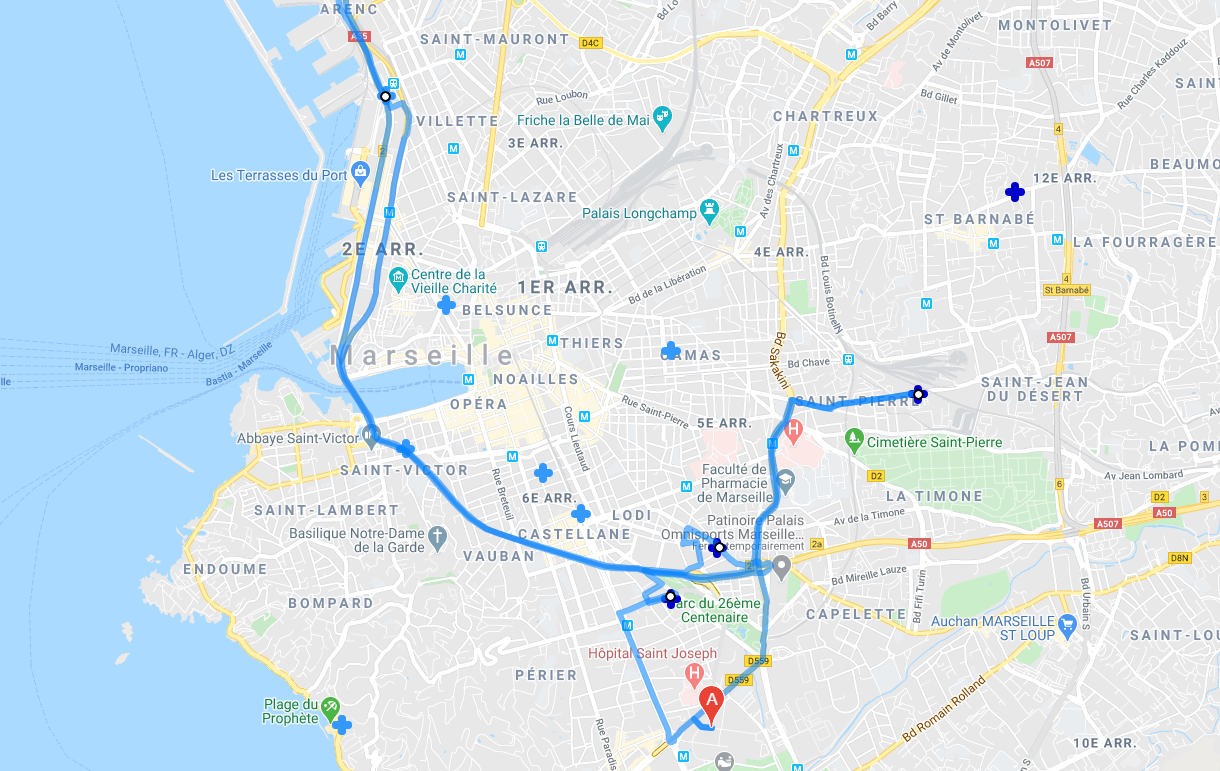
\includegraphics[width=0.85\textwidth]{completion marseille}
\medbreak
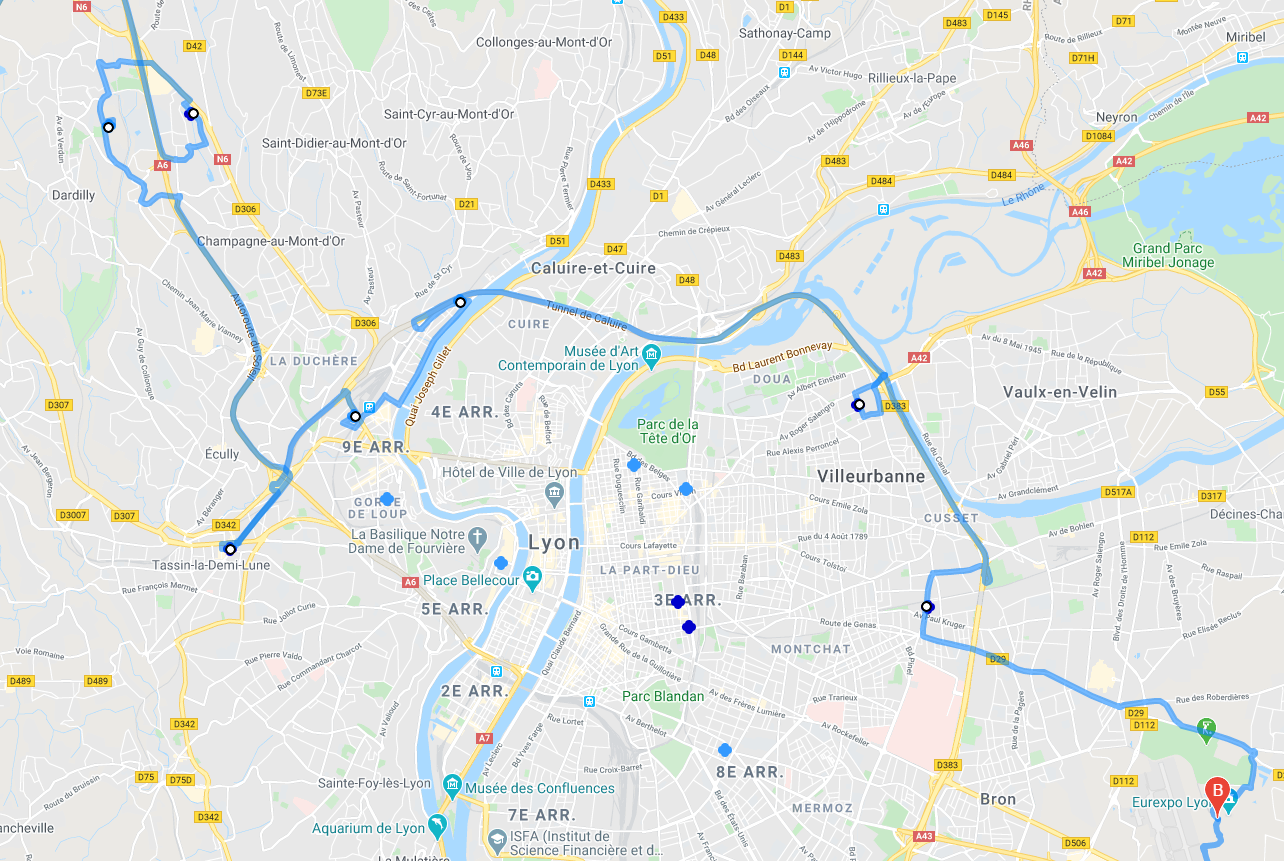
\includegraphics[width=0.85\textwidth]{completion lyon}
\end{center}
\end{figure}
\hyperlink{Ref6}{Retour lecture}

\label{Ref1}
\newpage
\subsection{Tournée optimale - D'autres exemples}
\hypertarget{Ref7}{}

\begin{figure}[H]
\caption{Tournée optimale dans Toulouse, à pied}
\begin{center}
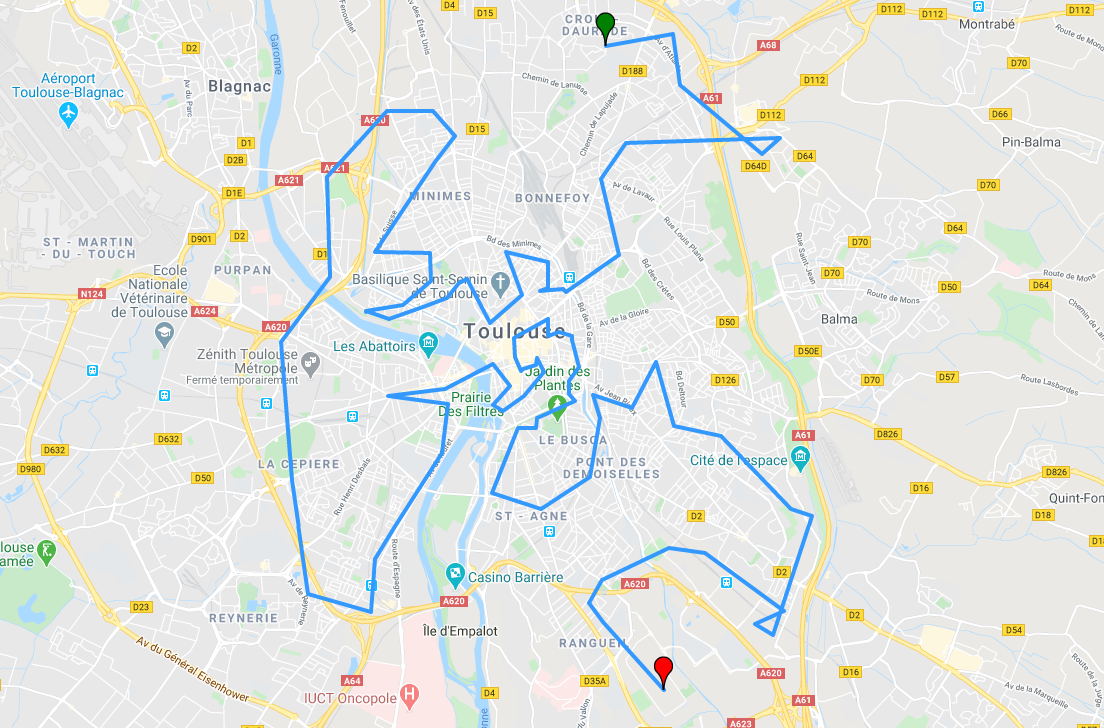
\includegraphics[width=0.95\textwidth]{toulouse walking}
\end{center}
\end{figure}

Remarque : impossible d'afficher tous les itinéraires à pied sur une même page, on voit donc les adresses reliées par des lignes, mais l'ordre optimal de passage a été calculé en utilisant les durées de trajets à pied fournies par google maps.
\hyperlink{Ref8}{Retour lecture}




\newpage
\hypertarget{Ref1}{}
\subsubsection{Autres exemples - Clustering d'adresses}
\begin{figure}[H]
\caption{Nouvelle Aquitaine - 91 adresses}
\begin{center}
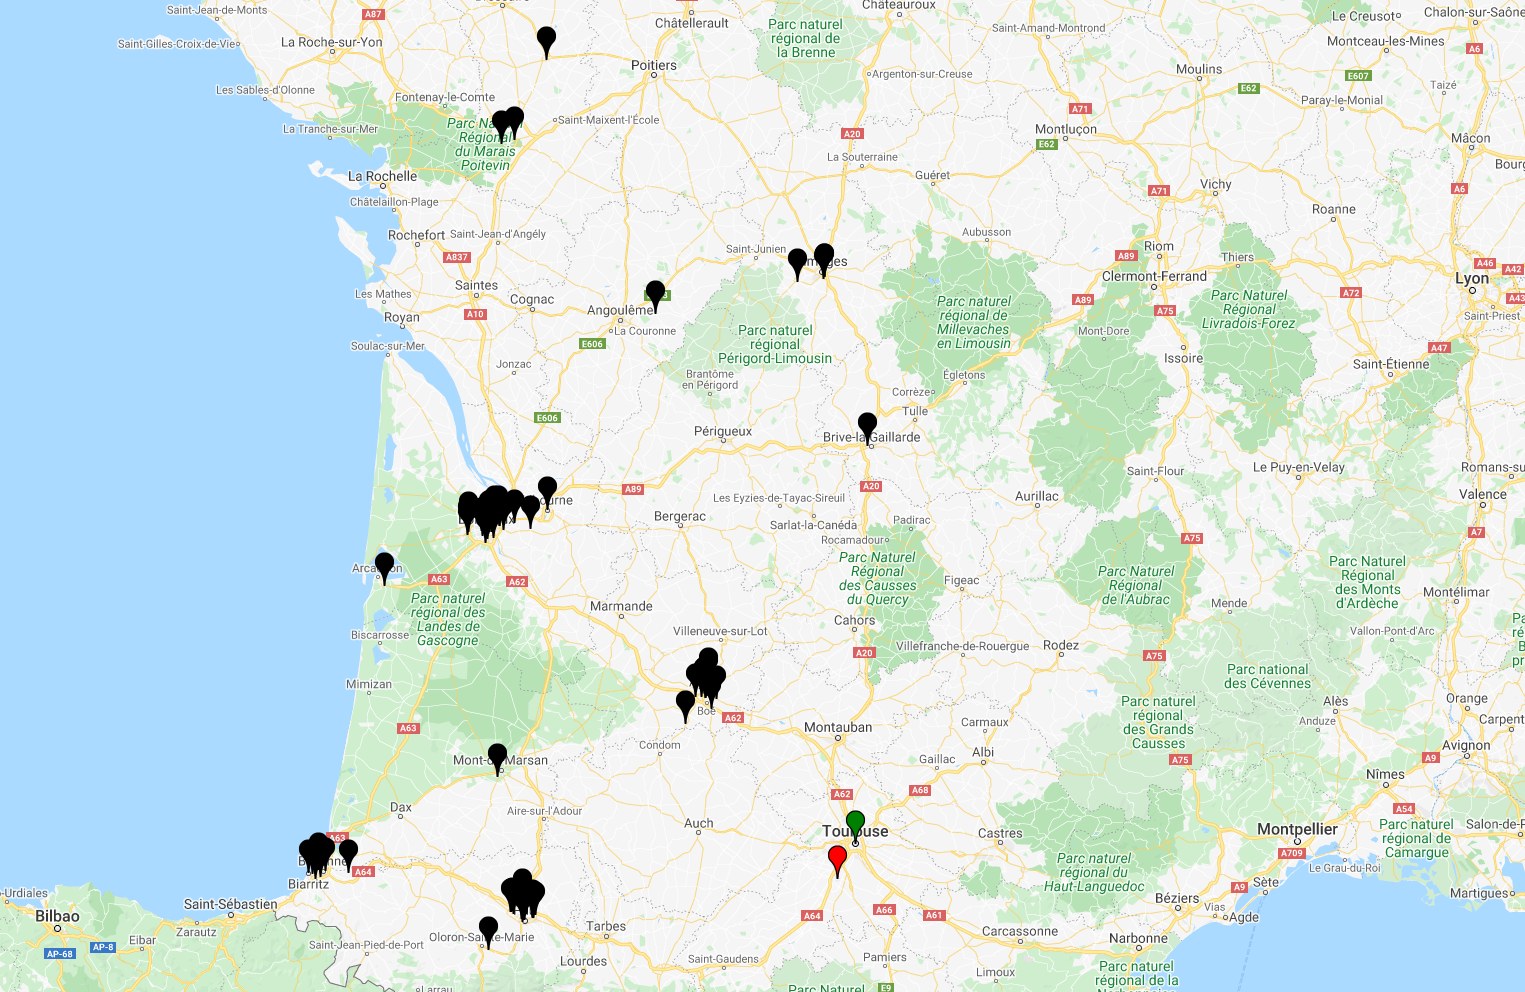
\includegraphics[width=0.99\textwidth]{NA_adresses}
\end{center}
\end{figure}

\begin{figure}[H]
\caption{Nouvelle Aquitaine - Clustering}
\begin{center}
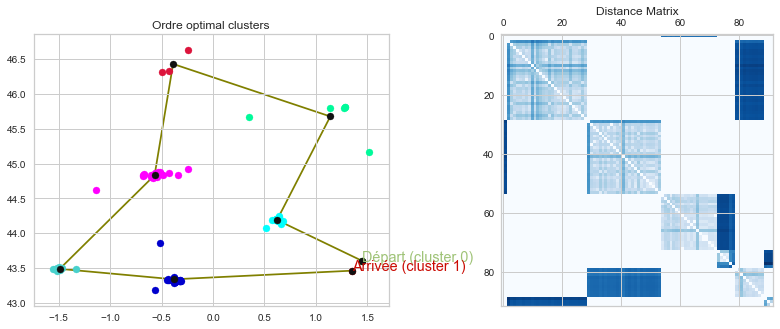
\includegraphics[width=0.99\textwidth]{NA_ordre_cluster_distance_matrix}
\end{center}
\end{figure}


\begin{figure}[H]
\caption{Nouvelle Aquitaine - Calcul des entrées/sorties}
\begin{center}
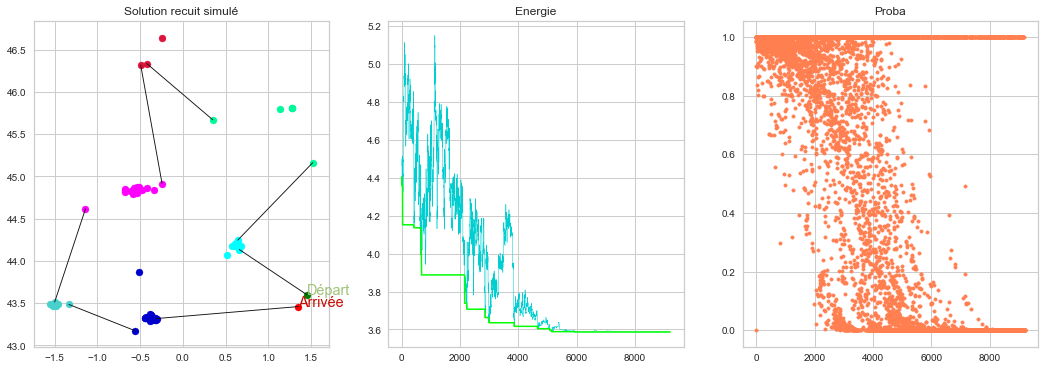
\includegraphics[width=0.99\textwidth]{NA_entrees_sorties}
\end{center}
\end{figure}

\begin{figure}[H]
\caption{Nouvelle Aquitaine - Trajet final - 90 adresses}
\begin{center}
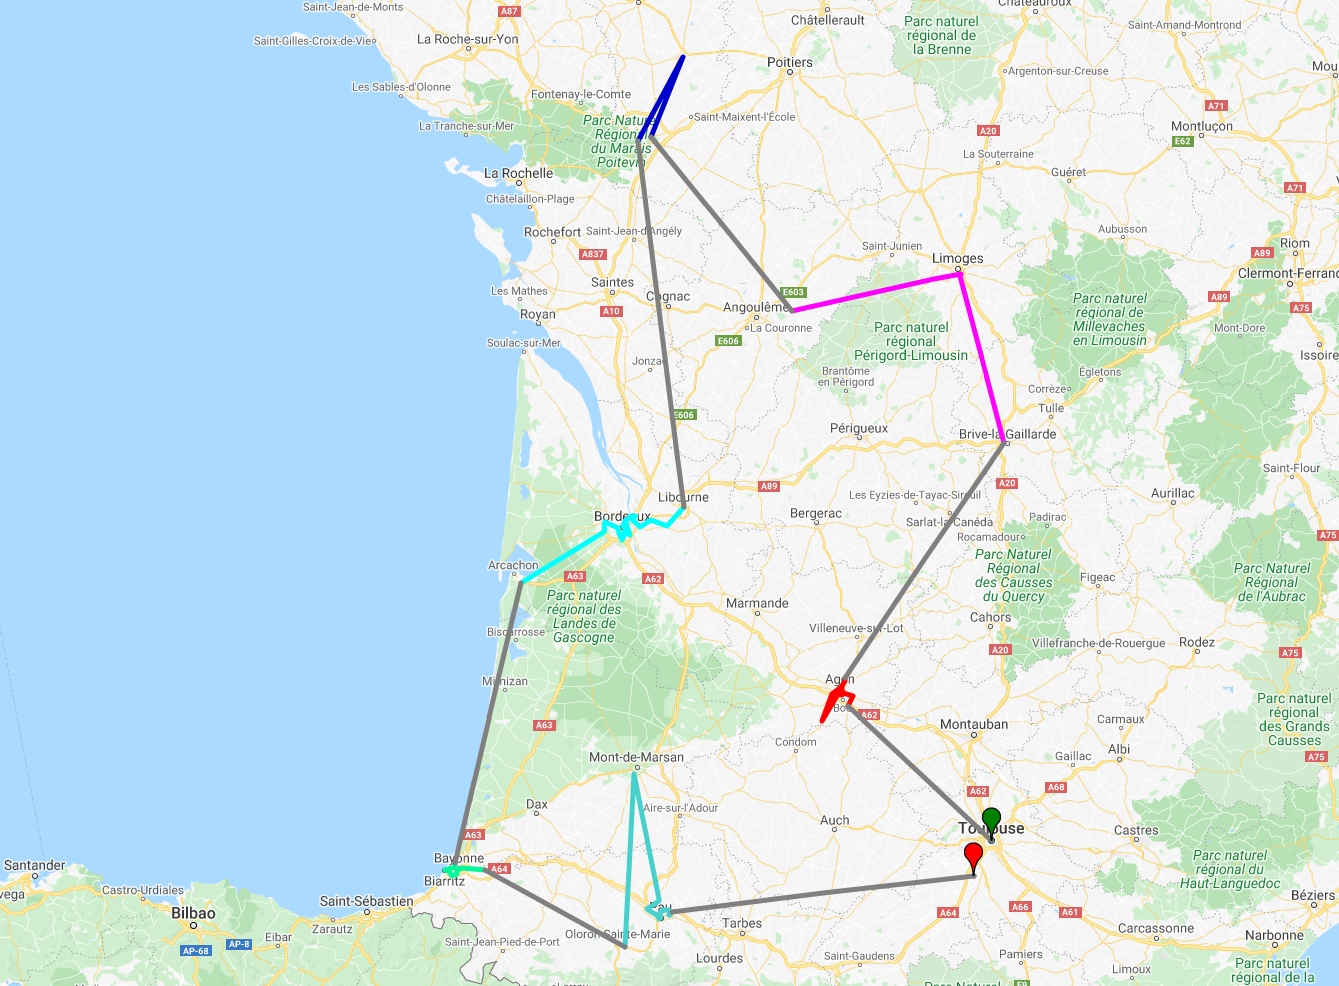
\includegraphics[width=0.99\textwidth]{NA_trajet_final}
\end{center}
\end{figure}

\begin{figure}[H]
\caption{Nouvelle Aquitaine - Zoom clusters importants}
\begin{center}
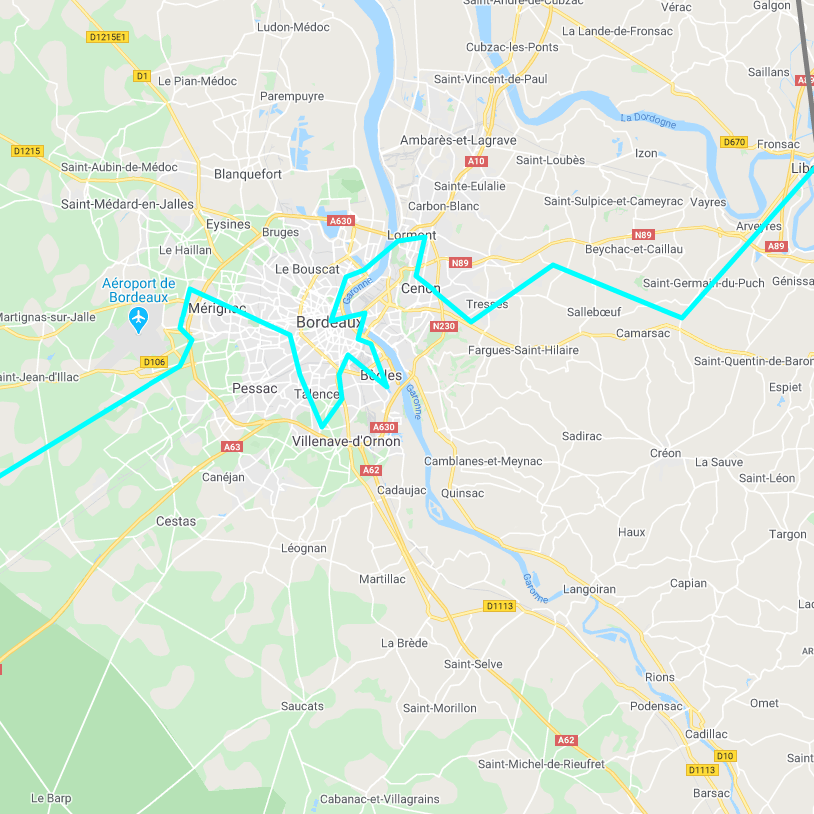
\includegraphics[width=0.32\textwidth]{NAcluster1}
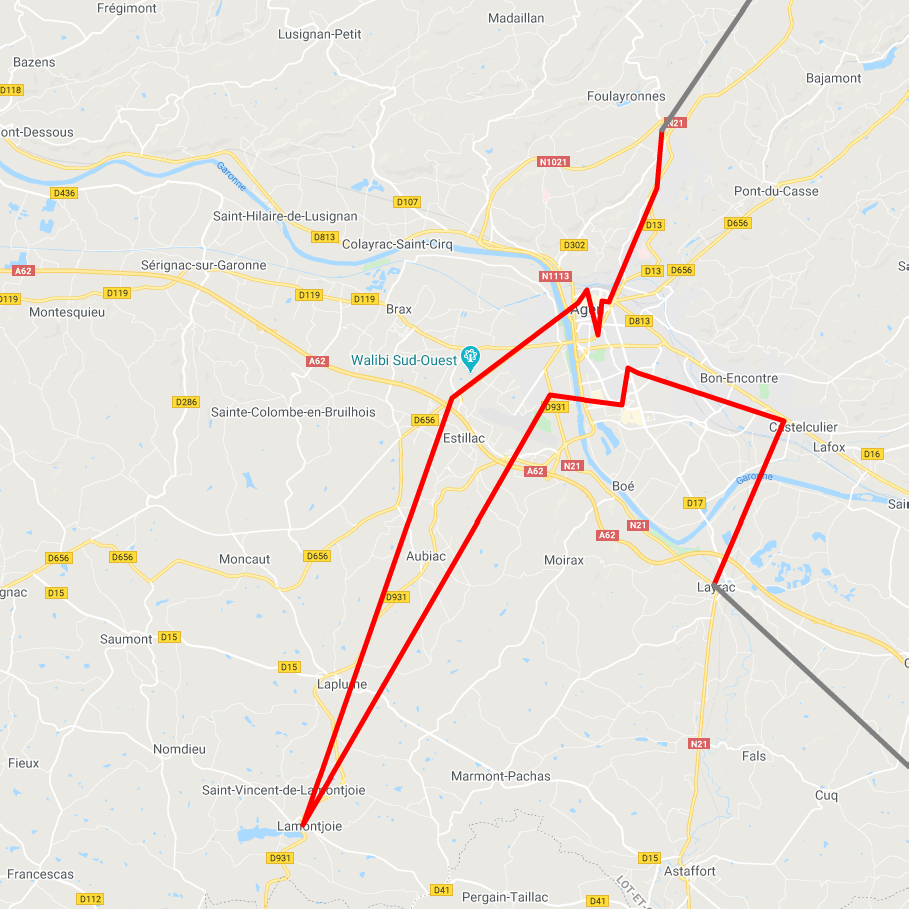
\includegraphics[width=0.32\textwidth]{NAcluster2}
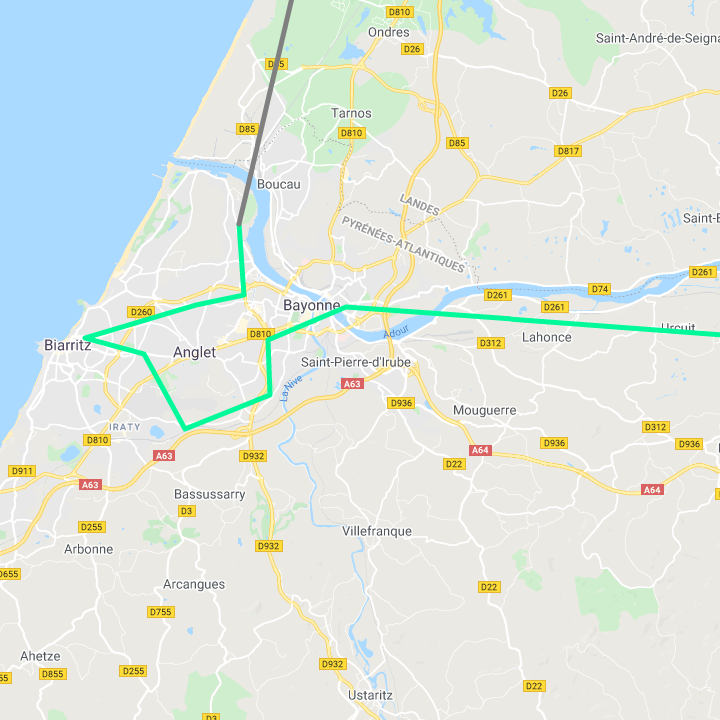
\includegraphics[width=0.32\textwidth]{NAcluster3}
\end{center}
\end{figure}

\hyperlink{Ref2}{Retour lecture}


\subsection{Optimisation répartition tâches}
\hypertarget{Ref10}{}
\begin{code}
DONNEES :
Charge totale de travail   : 1307 h pour 210 tâches avec 15 compétences possibles. 
							 ( 6 h/tâche).
Disponibilités totales     : 1398 h réparties sur 40 personnes 
							 ( 34 h/personne).
Approche choisie : 1

SORTIE :
Total heures non assignées : 0.0
Niveau moyen de spécialisation pour une heure travaillée : 0.98 / 3
Niveau moyen de spécialisation général : 0.2 / 3

Niveau moyen de compétence pour une heure travaillée     : 1.64 / 3
Niveau moyen de compétence général : 0.55 / 3

Statut résolution : Optimization terminated successfully.
Méthode de résolution      : interior-point
fonction objectif          : -2141.9999996335127
\end{code}
\begin{figure}[H]
\begin{center}
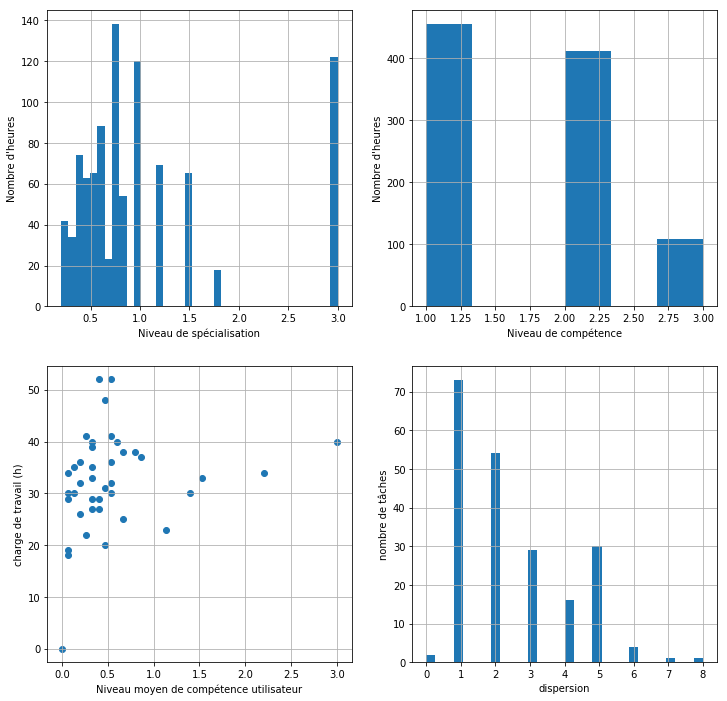
\includegraphics[width=0.85\textwidth]{SADT1}
\end{center}
\end{figure}



Dans cet exemple, on a simulé un problème de "grande taille" : beaucoup d'utilisateurs, de tâches, de projets. A priori ce programme devrait être utilisé principalement dans des dimensions plus petites.\\
Lorsque la dimension devient trop grande, l'algorithme du simplexe fournit dans la librairie scipy échoue à la résolution du problème, on relance donc en utilisant la méthode des points intérieurs.

Cette méthode a l'avantage de fonctionner même en grande dimension, mais alors la forme de la solution est différente. Cela nous d'ailleurs indique que la solution n'est pas unique.\\
L'inconvénient majeur de la solution fournie par les points intérieurs est qu'elle a tendance à attribuer les heures d'une même tâche à plusieurs utilisateurs (histogramme en bas à droite), ce qui dans la réalité n'est pas une bonne chose. Il est préférable qu'une seule personne se charge de dessiner les plans plutôt que 3.\\
Cela dépend bien sûr aussi des données, mais pour tenter de fournir la meilleure solution à l'utilisateur, j'ai choisi de résoudre le problème en utilisant le simplexe, et à défaut de succès, les points-intérieurs.

\hyperlink{ref12}{Retour lecture}

\newpage
\subsection{Emploi du temps}
\hypertarget{ref13}{}

\begin{code}
class Planning:
    # Création de l'objet
    def __init__(self, nom_utilisateur, id_utilisateur, plagehoraire_filename):
    
    # Pour changer les paramètres d'optimisation :
    def setPenalties(self, new_penalties):
    
    # Ajout des tâches à planifier
    def addTasks(self, df_tasks):
    
    # Calcul de la base de planning et des potentiels initiaux
    def initialise(self, DATE_DEBUT, DATE_FIN):
    # Ajout d'impératifs à prendre en compte
    def addImperatifs(self, df_imperatifs):
    
    # (maths) Met à jour les potentiels s'il y eu des changements
    def UpdateScores(self):
    
    # Propose un arrangement voisin des taches et stocke ses potentiels
    #Affiche les scores pour les différents indicateurs :
    def showScores(self):
    
    # (maths) Propose un arrangement voisin des taches et stocke ses potentiels
    def buildVoisin(self):
    
    # (maths) Remplace l'arrangement courant par l'arrangement voisin
    def replace(self):
    # (maths) Stocke l'arrangement conduisant à l'énergie totale la plus faible
    def replaceMin(self):
    
    # (maths) Remplace l'arrangement courant par l'arrangement "minimal" rencontré
    def applyMin(self):
    
     # (maths) Renvoie les potentiels de l'arrangement courant ou voisin selon la valeur du paramètre voisin
    def getPotentiels(self, voisin=False):
    
    # Exporte le planning en fichier excel et retourne le dataframe correspondant
    def makePlanning(self,to_file=False):
    
    # Fait l'inventaire des tâches non planifiées
    def notScheduled(self):
    
    
    
# TACHES MULTI-UTILISATEUR
# (maths)
def proj1(t,d):

# (maths)
def proj2(t,Is):

# (maths)
def h(t,Is):

#Planifie les tâches multi-utilisateurs à l'aide des 3 fonctions ci-dessus
def planifieTMU(TC,  DATE_DEBUT, DATE_FIN, plannings, maxiter = 100):


#AUTRES FONCTIONS :

#Calcule la base du planning, supprime les plages horaires < LONGUEUR MIN
def CalculBasePlanning(plagehoraire_filename, DATE_DEBUT, DATE_FIN, LONGUEUR_MIN = 0.5):


#Reconstruit la base en prenant en compte des impératifs
def addImperatifs(base, imp, LONGUEUR_MIN = 0.5):


# (maths) Permute deux taches dans une liste de tache
def permuteTasks(tasks):


# Découpe des tâches en morceaux n'excédant pas une durée choisie (mod_lenght en heure)
# ----> Avec mod_lenght = 1, une tâche de 3h30 est découpée
#       en 3 morceaux d'une heure et 1 d'une demi-heure
def split_tasks(Tasks, mod_lenght = 1):

\end{code}



\hyperlink{ref14}{Retour lecture}

\end{document}
